% Options for packages loaded elsewhere
\PassOptionsToPackage{unicode}{hyperref}
\PassOptionsToPackage{hyphens}{url}
%
\documentclass[
]{book}
\usepackage{amsmath,amssymb}
\usepackage{lmodern}
\usepackage{iftex}
\ifPDFTeX
  \usepackage[T1]{fontenc}
  \usepackage[utf8]{inputenc}
  \usepackage{textcomp} % provide euro and other symbols
\else % if luatex or xetex
  \usepackage{unicode-math}
  \defaultfontfeatures{Scale=MatchLowercase}
  \defaultfontfeatures[\rmfamily]{Ligatures=TeX,Scale=1}
\fi
% Use upquote if available, for straight quotes in verbatim environments
\IfFileExists{upquote.sty}{\usepackage{upquote}}{}
\IfFileExists{microtype.sty}{% use microtype if available
  \usepackage[]{microtype}
  \UseMicrotypeSet[protrusion]{basicmath} % disable protrusion for tt fonts
}{}
\makeatletter
\@ifundefined{KOMAClassName}{% if non-KOMA class
  \IfFileExists{parskip.sty}{%
    \usepackage{parskip}
  }{% else
    \setlength{\parindent}{0pt}
    \setlength{\parskip}{6pt plus 2pt minus 1pt}}
}{% if KOMA class
  \KOMAoptions{parskip=half}}
\makeatother
\usepackage{xcolor}
\usepackage{longtable,booktabs,array}
\usepackage{calc} % for calculating minipage widths
% Correct order of tables after \paragraph or \subparagraph
\usepackage{etoolbox}
\makeatletter
\patchcmd\longtable{\par}{\if@noskipsec\mbox{}\fi\par}{}{}
\makeatother
% Allow footnotes in longtable head/foot
\IfFileExists{footnotehyper.sty}{\usepackage{footnotehyper}}{\usepackage{footnote}}
\makesavenoteenv{longtable}
\usepackage{graphicx}
\makeatletter
\def\maxwidth{\ifdim\Gin@nat@width>\linewidth\linewidth\else\Gin@nat@width\fi}
\def\maxheight{\ifdim\Gin@nat@height>\textheight\textheight\else\Gin@nat@height\fi}
\makeatother
% Scale images if necessary, so that they will not overflow the page
% margins by default, and it is still possible to overwrite the defaults
% using explicit options in \includegraphics[width, height, ...]{}
\setkeys{Gin}{width=\maxwidth,height=\maxheight,keepaspectratio}
% Set default figure placement to htbp
\makeatletter
\def\fps@figure{htbp}
\makeatother
\setlength{\emergencystretch}{3em} % prevent overfull lines
\providecommand{\tightlist}{%
  \setlength{\itemsep}{0pt}\setlength{\parskip}{0pt}}
\setcounter{secnumdepth}{5}
\ifLuaTeX
  \usepackage{selnolig}  % disable illegal ligatures
\fi
\usepackage[]{natbib}
\bibliographystyle{plainnat}
\IfFileExists{bookmark.sty}{\usepackage{bookmark}}{\usepackage{hyperref}}
\IfFileExists{xurl.sty}{\usepackage{xurl}}{} % add URL line breaks if available
\urlstyle{same} % disable monospaced font for URLs
\hypersetup{
  pdftitle={Biology 125 Summer Lab Manual},
  hidelinks,
  pdfcreator={LaTeX via pandoc}}

\title{Biology 125 Summer Lab Manual}
\author{}
\date{\vspace{-2.5em}2022-08-22}

\begin{document}
\maketitle

{
\setcounter{tocdepth}{1}
\tableofcontents
}
\hypertarget{welcome}{%
\chapter*{Welcome}\label{welcome}}
\addcontentsline{toc}{chapter}{Welcome}

To your Biology 125 Labs for Biology for Science Majors II!

\textbf{First}, a few important and relevant links\ldots{}

\begin{itemize}
\tightlist
\item
  \href{https://canvas.ubc.ca/courses/94573}{Canvas course shell}
\item
  \href{https://canvas.ubc.ca/courses/94573/files/20871008}{Syllabus}
\end{itemize}

\textbf{Second}, some key pieces of information for how labs will be run this term\ldots{}

The following pages detail how labs, assignments, and absences will be handled. In addition to the content here, the lab manual, assignments, quizzes, and additional resources are all supplied on Canvas so take some time to look over the information.

If in doubt about course policies, refer to your syllabus or talk to your TA. To get started read through your course syllabus and the lab manual.

Above all, have fun this term and enjoy the process of science!

Sincerely,

Dr.~Tristyn Hay

\hypertarget{labs}{%
\section*{Labs}\label{labs}}
\addcontentsline{toc}{section}{Labs}

Similar to term 1, labs will be alternating between on-campus and online, with some online labs being conducted in Zoom during your regular scheduled lab section. In order to be successful this term please pay attention to your syllabus where you can find your schedule, mark breakdown, missed lab policy, and all lab requirements for your BIOL125 lab. You will need the information found in this syllabus to be able to answer the Introductory Quiz on canvas. Students will not be excused of any missed or late assignments due to being "unaware" of these policies so be sure you reference this information often.

Your first lab, Lab 1, is on campus - meaning that you complete your lab in the lab - with the relevant material being posted on Canvas. You will have the opportunity to meet your TA and the other students registered in your lab section. This lab will be a very important lab as you will have your partner assigned to you and will be setting up for an experiment. For in-person labs, it is vital that you attend the lab for which you are registered - check your registration online to be sure of where you are supposed to be!

Your second lab, Lab 2, will be online - meaning you will work through your lab via Zoom during your regular scheduled lab time. Your TA will be navigating you through your entire lab during your regular scheduled lab time.

During the on campus labs you may bring a lab coat but this is not required. Closed toed shoes and pants are required for this lab and your TA will turn you away if you are not in proper attire. Any goggles and gloves will be provided in lab.

\hypertarget{assignments}{%
\section*{Assignments}\label{assignments}}
\addcontentsline{toc}{section}{Assignments}

See Canvas for due dates.

All assignments, even those worked on as a group, will need to be submitted individually unless directed to do so by your TA.

Failure to submit an assignment will result in a mark of 0 for that assignment. No exceptions!

Please be sure you have not only submitted assignments on time but that you have double-checked they have been uploaded properly.

\hypertarget{absences}{%
\section*{Absences}\label{absences}}
\addcontentsline{toc}{section}{Absences}

Pay attention to your absence scores - see syllabus for details. Students receiving an absence score over 5 will fail the lab. This applies to both on campus and online assignments. If an assignment is not submitted it counts as an absence. Excused absences get a score of 1 and unexcused a score of 2.5.

Absences can only be excused by the lab coordinator and not your TA.

\hypertarget{copyright}{%
\section*{Copyright}\label{copyright}}
\addcontentsline{toc}{section}{Copyright}

This work is licenced under the Creative Commons \href{https://creativecommons.org/licenses/by-nc-sa/4.0/}{Attribution-NonCommercial-ShareAlike 4.0 International (CC BY-NC-SA 4.0)}

Please use the following for citing this document

Hay, T., Vis-Dunbar, M. (2021). \emph{Biology 125 Lab Manual}. \url{https://ubco-biology.github.io/BIOL-125-Lab-Manual/}

All source files are available \url{https://github.com/ubco-biology/BIOL-125-Lab-Manual}.

\hypertarget{ubco-biology-open-materials}{%
\section*{UBCO Biology open materials}\label{ubco-biology-open-materials}}
\addcontentsline{toc}{section}{UBCO Biology open materials}

This resource is part of a larger project to host UBCO Biology lab materials in an open, accessible format.

All BIOL open materials can be found at \url{https://ubco-biology.github.io/}

\hypertarget{conventions}{%
\section*{Conventions}\label{conventions}}
\addcontentsline{toc}{section}{Conventions}

Information relevant to lab logistics and grading.

Further insights or notes on presented materials.

Highlights and key take aways.

Optional material that dives deeper into a presented concept.

\hypertarget{part-lab-1}{%
\part*{Lab 1}\label{part-lab-1}}
\addcontentsline{toc}{part}{Lab 1}

\hypertarget{welcome-1}{%
\chapter*{Welcome}\label{welcome-1}}
\addcontentsline{toc}{chapter}{Welcome}

\emph{Last updated 2022-08-22}

Welcome to your first Biology 125 Lab for Biology for Science Majors II!

For your first week your TA will spend a bit of time going over the lab schedule and mark breakdown, along with some safety information you will need to work in this space safely and professionally. Your TA will also provide you with their contact information along with office hours and location. It is your responsibility to ensure you have this information readily available. Your TA will then get you going on your first project!

Labs will run in both an online and on-campus format. Please be mindful of the schedule.Failure to attend an on-campus lab due to students not reading their syllabus and schedule thoroughly will result in a mark of zero for that lab and an absence score of 2.5 (please see syllabus as you cannot exceed a score of 5 as this results in failing the lab).

\hypertarget{your-first-project}{%
\section*{Your first project}\label{your-first-project}}
\addcontentsline{toc}{section}{Your first project}

After this brief introduction you will get into pairs (with one group of 3 in uneven class sizes) and your TA will assign you and your partner(s) an environmental problem. Together you will design an experiment in order to try and solve the problem at hand. However due to the time constraints over the summer we will be unable to run the experiments in lab but you will be given a data set in which to complete the remaining assignments for the labs.

During the on-campus labs you may bring a lab coat but this is not required. Closed toed shoes and pants are required for this lab and your TA will turn you away if you are not in proper attire.Any goggles and gloves will be provided in lab.

\hypertarget{but-first}{%
\section*{But first\ldots{}}\label{but-first}}
\addcontentsline{toc}{section}{But first\ldots{}}


\includegraphics{images/img-1.png}

Did you know this little guy is actually real??? Anyone guess what these guys are called?

If you have a guess send an email to your TA or feel free to just say hello.

\hypertarget{research-project-part-1}{%
\chapter*{Research Project: Part 1}\label{research-project-part-1}}
\addcontentsline{toc}{chapter}{Research Project: Part 1}

\hypertarget{farmer-in-need-of-land-recommendations-needed}{%
\section*{Farmer in need of land: Recommendations needed}\label{farmer-in-need-of-land-recommendations-needed}}
\addcontentsline{toc}{section}{Farmer in need of land: Recommendations needed}

Farmer Elliot is looking to acquire a 20-acre farm to grow mung beans. Farmer Elliot has some basic knowledge of farming as he did some residential gardening in the city and thus understands the basic requirements of plants but has limited knowledge of growing mung beans.

You might be asking why Farmer Elliot is pursuing this when without the needed knowledge ahead of time? Let's just leave it as Farmer Elliot is a "act now think later" kind of person.

\begin{figure}
\centering
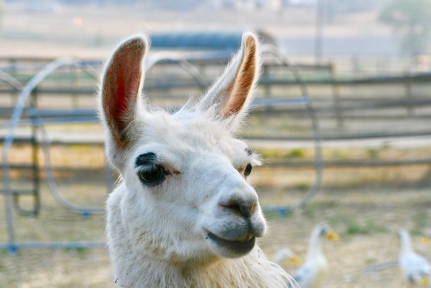
\includegraphics{images/img-2.png}
\caption{Elliot. The character behind the farmer. Find more pics of Elliot in your syllabus!}
\end{figure}

\hypertarget{finding-property}{%
\section*{Finding property}\label{finding-property}}
\addcontentsline{toc}{section}{Finding property}

In order to start their search Farmer Elliot has enlisted the help of a real-estate company - "llamaste Realty". Their real-estate company has shown them three properties thus far.

\hypertarget{property-1}{%
\subsection*{Property 1}\label{property-1}}
\addcontentsline{toc}{subsection}{Property 1}

\begin{figure}
\centering
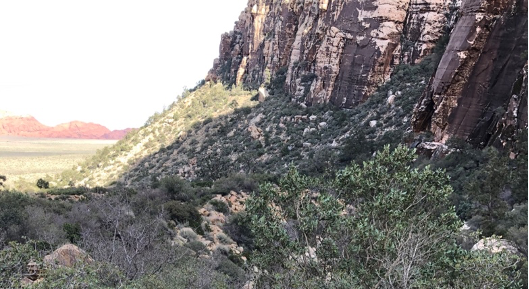
\includegraphics{images/prop-1.png}
\caption{Property 1.}
\end{figure}

This property has 19-acres of flat useable land and is situated next to the base of a large mountain. This land comes with fully automated irrigation and a small one-bedroom home. Though this land is start up ready, Farmer Elliot is concerned that the property may not have enough hours of sunlight due to its proximity to the base of the mountain.

In order to help determine if this is a viable option for his mung bean farm, Farmer Elliot will need to know how many hours of sunlight is required for optimum mung bean germination and growth.

\hypertarget{property-2}{%
\subsection*{Property 2}\label{property-2}}
\addcontentsline{toc}{subsection}{Property 2}

\begin{figure}
\centering
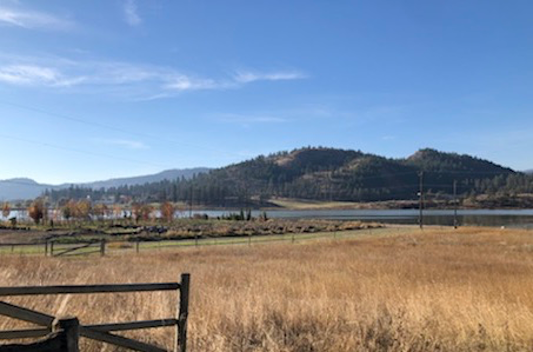
\includegraphics{images/prop-2.png}
\caption{Property 2.}
\end{figure}

This property has 21 acres of land with 3 acres designated to residential space and the remaining land is useable agricultural acreage. Running parallel to the longest section of this property is a small alkaline lake. Farmer Elliot has been informed that the adjacent alkali lake has, on average, a salinity concentration ranging from 0-5\%.

Not knowing if salinity has an impact on germination and growth of munch beans Farmer Elliot is not sure if this is the best property for his endeavor.

\hypertarget{property-3}{%
\subsection*{Property 3}\label{property-3}}
\addcontentsline{toc}{subsection}{Property 3}

\begin{figure}
\centering
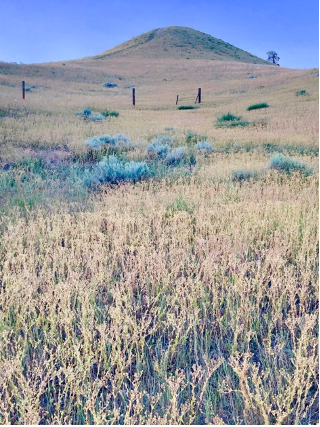
\includegraphics{images/prop-3.png}
\caption{Property 3.}
\end{figure}

Property \#3 is located at a much higher elevation than the other properties and located in a very different biogeoclimatic zone than what Farmer Elliot is familiar with and the differences in mineral content and soil texture in this area results in soil pH levels ranging between 6.2-7.2. It comes with a 2-bedroom home and 20 acres of useable ready to grow acreage.

This property appears ideal but Farmer Elliot is unsure if this pH range is tolerable for mung bean germination and growth.

\hypertarget{your-role}{%
\section*{Your Role}\label{your-role}}
\addcontentsline{toc}{section}{Your Role}

In order to better inform Farmer Elliot's decision Farmer Elliot has hired you and your partner as consultants.

Your TA will assign a specific property listing to you and your partner and you will be tasked with designing an experiment to test the specified variable on both mung bean germination and growth.Due to time constraints over the summer months we will not be running an experiment but rather you, and your partner, will be provided a data set to work through your recommendation report for your client Farmer Elliot.

To help you in this endeavour, you may wish to review the content from BIOL116 on experimental design -- \href{https://ubco-biology.github.io/BIOL-116-Lab-Manual/designing-the-experiment.html}{Designing the Experiment}.

\hypertarget{research-data-management}{%
\chapter*{Research Data Management}\label{research-data-management}}
\addcontentsline{toc}{chapter}{Research Data Management}

How we organize and store our research data - Research Data Management or RDM for short - is a critical component of reproducibility and transparency in the sciences.

In BIOL116, you were introduced to best practices in file naming. You may wish to \href{https://ubco-biology.github.io/Procedures-and-Guidelines/file-naming.html}{review that content here}. In this lab, you'll be looking at best practices in directory structure management; that is, how we organize our individual files. Just like with file naming conventions, it is extremely important that our files are organized in a way that logically reflects the structure of our project and can be easily navigated with computation tools, allowing for, at a minimum, \href{https://ubco-biology.github.io/BIOL-116-Lab-Manual/computational-reproducibility.html}{computational reproducibility}. There is also an increased need to provide documentation that describes the chosen structure; in fact, the more complex a project becomes, the more this documentation is important.

So, before proceeding, review the content in the Procedures and Guidelines Document under \href{https://ubco-biology.github.io/Procedures-and-Guidelines/directories.html}{Directories} and \href{https://ubco-biology.github.io/Procedures-and-Guidelines/directory-structures.html}{Directory Structures}.

\textbf{After reviewing this content complete the short quiz on Canvas}

\hypertarget{research-question}{%
\chapter*{Research Question}\label{research-question}}
\addcontentsline{toc}{chapter}{Research Question}

First things first, we need a good research question.

In BIOL116 you were introduced to experimental design and hypothesis testing. One of the things we didn't touch on in great detail was how to develop a research question.

How you formulate your research question will impact what you study and how you conduct that study.

When we think about transparency and reproducibility in research design and implementation, every step we take and every decision we make is predicated on earlier decisions; and things begin with a research question. Well, to be fair, developing a research question is an iterative process, but it underpins so many future decisions - it will inform your hypothesis -- after all, your hypothesis is the testable statement that addresses your research question -- which will then inform your study design and so on. So, we shouldn't gloss over its importance!

\hypertarget{a-good-research-question}{%
\section*{A good research question}\label{a-good-research-question}}
\addcontentsline{toc}{section}{A good research question}

A good research question will help to limit many biases that Open Science is trying to combat in the conduct of research, including HARKing and making decisions after having looked at one's data.

A good research question is primarily informed by two things:

\begin{itemize}
\tightlist
\item
  Research done to date that has addressed this problem.
\item
  The problem at hand
\end{itemize}

\hypertarget{background}{%
\section*{Background}\label{background}}
\addcontentsline{toc}{section}{Background}

\hypertarget{consulting-the-literature}{%
\subsection*{Consulting the literature}\label{consulting-the-literature}}
\addcontentsline{toc}{subsection}{Consulting the literature}

Consulting research done to date will allow you to see how this or similar questions have been addressed by other researchers. Novel ways of addressing the same question are important to move science forward; consulting previous research will help to identify gaps that are opportunities for these novel approaches.

At the same time, consistency in methodology underpins reproducibility, and it's consequently just as important to test the same the questions with the same methods in both similar and novel populations as previous research has done, helping to build a body of evidence and identify if earlier findings are generalizable to other populations.

\hypertarget{the-problem-at-hand}{%
\subsection*{The problem at hand}\label{the-problem-at-hand}}
\addcontentsline{toc}{subsection}{The problem at hand}

The problem at hand will come with certain known and unknown elements. In this assignment, depending on the plot of land that you're looking at, you already know certain things about the soil chemistry, geological features or water sources of a given plot.

It is the unknown elements -- or a portion of the unknown elements -- that your research question will try and address. In this instance, how these factors will impact mung bean production.

A research question that asks

\begin{quote}
What is the impact of fertilizer x on the growth of mung beans?
\end{quote}

would seem a reasonable first attempt at addressing one potential issue at hand. However, it doesn't give a clear definition of what we're measuring as either a dependent or independent variable.

Since the research question informs the hypothesis, which then guides your design, you're leaving yourself with a lot of wriggle room here further down the line.

\hypertarget{phrasing}{%
\section*{Phrasing}\label{phrasing}}
\addcontentsline{toc}{section}{Phrasing}

\hypertarget{a-testable-question}{%
\subsection*{A testable question}\label{a-testable-question}}
\addcontentsline{toc}{subsection}{A testable question}

Using the word \textbf{what} re-enforces this less than concise formulation of the research question. In fact, predicating your question with \textbf{what} or \textbf{why} doesn't allow your question to ask exactly what you need it to ask.

In experimental design, we're testing for relationships - asking "is there a relationship?". In fact, we're asking a question that allows for the proposal of a hypothesis; a prediction of what that relationship might be. So, we should think about how we can ask a question that reflects the test or experiment we're planning.

\hypertarget{a-succinct-question}{%
\subsection*{A succinct question}\label{a-succinct-question}}
\addcontentsline{toc}{subsection}{A succinct question}

In addition to re-framing our question to one which is phrased as a testable question, we want to clearly articulate our population of interest and our main variables of interest. When phrased as

\begin{quote}
What is the impact of fertilizer x on the growth of mung beans?
\end{quote}

the variables ostensibly include fertilizer and plant growth. But plant growth is more nuanced than this, and our study might be too. In fact, arguably, plant growth is not a variable, but a composite of variables; so, we should ask ourselves, "what do we mean by growth? What about growth are we interested in? Germination rate, germination survival, biomass, height, flower set, fruit set?"

Defining the scope of your population and variables is a key consideration when developing a research question; defining these early means that you won't be asking these questions later, once you've already started to collect, or work with, your data.

So, ultimately, we want a question that:

\begin{itemize}
\tightlist
\item
  Is testable;
\item
  Clearly identifies our population;
\item
  Clearly identifies our primary variables of interest; and
\item
  Is concise
\end{itemize}

\hypertarget{an-example}{%
\section*{An Example}\label{an-example}}
\addcontentsline{toc}{section}{An Example}

Let's say our farmer is concerned primarily about fruit set. It seems reasonable then to test for fruit set. Again, fruit set could be defined in many ways - average biomass per fruit, average count per plant etc. And we may or may not be interested in each of these outcomes. In either case, a more concise, testable research question might then look like

\begin{quote}
Will the application of fertilizer x increase the quantity of fruit set of Vigna radiata?
\end{quote}

Not only can we test this, it identifies exactly what we're interested in testing, and it's concise, which means that we can then readily propose a hypothesis and null hypothesis to address it:

\begin{itemize}
\tightlist
\item
  Ho: fertilizer x will increase the quantity of fruit set of Vigna radiata.
\item
  Ha: fertilizer x will have no impact on the quantity of fruit set of Vigna radiata.
\end{itemize}

Reproducibility, meta-analyses, and the evidence base

When we reproduce a study, we always know that there is a chance of error or bias resulting from our sample not being truly representative of its population, for any number of reasons including sampling error, lack of power etc. This is why we should never rely on the findings of just one study.

A meta-analysis is a study of already conducted studies to try and determine if across a series of studies addressing the same research question there is enough agreement in the findings to accept one conclusion, even though this conclusion may be contradicted by individual studies.

Reproducibility enables this aggregation of findings, helping to sift through studies that have suffered from systematic error. To do this well, meta-analyses rely on documentation and homogeneity; studies that use similar methods, instruments, and techniques to address the same question and describe in detail how this was done. This is because comparing two studies of the same phenomenon with two different research questions and two different methodological approaches and data collection tools is extremely confounding and limiting.

Meta-analyses are based on extremely comprehensive literature reviews, reviews that attempt to uncover all literature -- published and unpublished -- addressing a given research question. Your research question not only informs your hypothesis and study design, it also frames your title and abstract, whether for a lab report, poster, or one day a manuscript. Expressing your research question in a way that clearly and succinctly outlines the variables you plan to test makes the inclusion of your results in a meta-analysis more likely, as your work will be more easily discovered and identified.

In fact, with this in mind, if you were conducting your mung bean research for a particular plot of land in a particular region, this might impact the variables you choose to work with, and you might end up with a still more concise research question that would allow for identification of potential homogeneity and then for comparing your data against other similar studies in a meaningful way. So, for example, in the Okanagan, your research question might be adjusted to

\begin{quote}
Will the application of fertilizer x increase the quantity of fruit set of Vigna radiata in a sandy loam soil of the BC Okanagan Valley?
\end{quote}

\hypertarget{assignment-lab-1}{%
\chapter*{Assignment: Lab 1}\label{assignment-lab-1}}
\addcontentsline{toc}{chapter}{Assignment: Lab 1}

Please use the following template for this assignment:

\href{https://osf.io/download/pxuy9}{20220628\_Lab01\_125\_Protocol-Assignment\_V1.docx} (17 KB)

\hypertarget{putting-it-into-practice}{%
\subsection*{Putting it into practice}\label{putting-it-into-practice}}
\addcontentsline{toc}{subsection}{Putting it into practice}

Drawing on what you learned in BIOL116 and after reviewing the content for this lab, this assignment asks you to articulate the key components of a protocol: a research question, hypothesis, and proposed study time line, as well as to describe the kind of data (variables as well as data types) you'll be collecting, how you'll be collecting it, and what you'll be doing with these data.

\hypertarget{part-lab-2}{%
\part*{Lab 2}\label{part-lab-2}}
\addcontentsline{toc}{part}{Lab 2}

\hypertarget{open-science}{%
\chapter*{Open Science}\label{open-science}}
\addcontentsline{toc}{chapter}{Open Science}

\emph{Last updated 2022-08-22}

This week's lab content is the second half of \href{https://ubco-biology.github.io/OS-Introduction/}{Open Science: An Introduction}.

You are asked to cover Parts 2 and 3, \href{https://ubco-biology.github.io/OS-Introduction/open-science-in-action-benefits.html}{Open Science in Action: Benefits}, and \href{https://ubco-biology.github.io/OS-Introduction/open-science-in-action-challenges.html}{Open Science in Action: Challenges}, respectfully.

The accompanying quiz can be found in \href{https://canvas.ubc.ca/courses/94573}{Canvas}.

\hypertarget{part-lab-3}{%
\part*{Lab 3}\label{part-lab-3}}
\addcontentsline{toc}{part}{Lab 3}

\hypertarget{research-project-part-2}{%
\chapter*{Research Project: Part 2}\label{research-project-part-2}}
\addcontentsline{toc}{chapter}{Research Project: Part 2}

\emph{Last updated 2022-08-22}

\hypertarget{rshiny-app}{%
\subsection*{RShiny App}\label{rshiny-app}}
\addcontentsline{toc}{subsection}{RShiny App}

For this on-campus lab, you will need to ensure you bring in your laptop in order to complete the Assignment. You and your partner will work through your data set in the lab. You will need the link below (also available on Canvas) in order to upload your data, set it into the RShiny App, and run the descriptive statistics.

\url{https://openscience.ok.ubc.ca/shiny/BIOL-116/}

Though you and your partner will be working through this data set together you will still need to upload independently. That is each person must upload a copy of the assignment or it will be marked as zero. NO EXCEPTIONS.

Your TA will assign you data to use for the assignment. Here are links to the data sets that will be used in this lab:

\begin{itemize}
\tightlist
\item
  \href{https://osf.io/download/pu6tb}{Property1\_Light\_GrowthRate}
\item
  \href{https://osf.io/download/a7qgj}{Property1\_Light\_Germination}
\item
  \href{https://osf.io/download/pf4ym}{Property2\_Salinity\_GrowthRate}
\item
  \href{https://osf.io/download/ak6cs}{Property2\_Salinity\_Germination}
\item
  \href{https://osf.io/download/5ravz}{Property3\_pH\_GrowthRate}
\item
  \href{https://osf.io/download/rsp6q}{Property3\_pH\_Germination}
\end{itemize}

\hypertarget{recommendation-report-rubric}{%
\section*{Recommendation Report Rubric}\label{recommendation-report-rubric}}
\addcontentsline{toc}{section}{Recommendation Report Rubric}

As we near completion of the research project, it is a good idea to get familiar with the format and expectations for your final Recommendation Report.

See \href{https://ubco-biology.github.io/BIOL-125-Lab-Manual-Summer/assignment-recommendation-report.html}{Lab 4} for an overview of the expectations of the Recommendation Report and to review the \href{https://ubco-biology.github.io/BIOL-125-Lab-Manual-Summer/recommendation-report-rubric-1.html}{grading rubric}.

\hypertarget{assignment-lab-3}{%
\chapter*{Assignment: Lab 3}\label{assignment-lab-3}}
\addcontentsline{toc}{chapter}{Assignment: Lab 3}

Download a copy of the assignment \href{https://osf.io/download/cr9py}{Lab\_3\_RShiny\_Assignment\_2}.

Use the \href{https://openscience.ok.ubc.ca/shiny/BIOL-116/}{RShiny App} to complete your assignment.

You may wish to refer back to the section on \href{https://ubco-biology.github.io/BIOL-116-Lab-Manual/preparing-your-data.html}{Preparing your data} from BIOL 116 and the chapter \href{https://ubco-biology.github.io/Procedures-and-Guidelines/tidy-data.html}{Tidy Data} in the Procedures and Guidelines document.

Upload your completed assignment to \href{https://canvas.ubc.ca/}{Canvas}

\textbf{Using R Scripts as an Alternative to RShiny}

If you are feeling ambitious and would like to try making plots, calculating descriptive statistics, and performing analyses using R instead of the RShiny App, some R scripts are provided in the \href{https://ubco-biology.github.io/BIOL-116-Lab-Manual/lab-7-activity.html}{Optional Deeper Dive here} in the BIOL 116 Lab manual for your use. These scripts align with the code used to produce figures, stats, and analyses in the RShiny App. However, by using these R Scripts you can edit code to customize the outputs (ie. change the fill colour on your figure etc.).

\emph{Keep in mind that there will be no additional support through TA's or instructors should you choose to use these scripts.}

\hypertarget{part-lab-4}{%
\part*{Lab 4}\label{part-lab-4}}
\addcontentsline{toc}{part}{Lab 4}

\hypertarget{animal-systems-i-part-one}{%
\chapter*{Animal Systems I: Part One}\label{animal-systems-i-part-one}}
\addcontentsline{toc}{chapter}{Animal Systems I: Part One}

\emph{Last updated 2022-08-22}

\hypertarget{overview-of-the-week}{%
\subsection*{Overview of the Week}\label{overview-of-the-week}}
\addcontentsline{toc}{subsection}{Overview of the Week}

The breakdown for this week's lab;

\begin{enumerate}
\def\labelenumi{\arabic{enumi}.}
\tightlist
\item
  You will be joining your lab mates and TA during your regular scheduled time but online
\item
  Your TA will go through a PowerPoint presentation online
\item
  You will be given time to review all material provided on Canvas
\item
  You must complete all quizzes for this week's lab provided on \href{https://canvas.ubc.ca/}{Canvas} due \textbf{before 11:59 pm on July 20th}
\item
  Your Recommendation Report Draft is due this week. Submit your draft \textbf{before 11:59 pm on July 18th} to avoid a late penalty or a zero!
\end{enumerate}

\textbf{Before lab} you will need to read through the information outlined below in Animal Systems Information for three phyla: Annelida, Mollusca and Arthropoda.

In this lab, you will be working your way through the material posted on Canvas online but during your scheduled lab time. Your TA will spend time going over a quick \href{https://osf.io/download/b2v8t}{PowerPoint presentation} regarding these animals. You will then need to spend a fair bit of time going through the different videos, images, and written material provided to ensure you have a solid grasp of these animals before coming to campus next week for your synchronous week. You must complete all quizzes associated with the animals found in animal systems I before \textbf{11:59 pm on July 20th}. Even though you will be getting together this week there is no reason you can't start reviewing all this information ahead of time so that you are better prepared to get through the material during your lab section.

\hypertarget{animal-systems-information}{%
\chapter*{Animal Systems Information}\label{animal-systems-information}}
\addcontentsline{toc}{chapter}{Animal Systems Information}

\hypertarget{phylum-annelida}{%
\subsection*{Phylum Annelida}\label{phylum-annelida}}
\addcontentsline{toc}{subsection}{Phylum Annelida}

\emph{Biology 125 Biology for Science Majors II Lab Manual. Written by Dr.~Tristyn Hay October, 2021. Some content provided by the University of British Columbia and Okanagan Biology Graduate Program students handbook The Fictional Animal Project: A Tool for Helping Students Integrate Body Systems. Adv. Physiol. Edu 41: 239-243 Blatch et al.~2017}

The phylum Annelida includes all segmented worms that have a coelom functioning as a hydrostatic skeleton. Other than the first and last portion, they are built on a pattern of repeated segments through which a ``one-way" digestive tract (mouth and anus), closed circulatory system (blood is completely enclosed in vessels), and nervous system pass. The annelids do not have specialized gas exchange structures, instead the blood vessels pass very close to the bodies surfaces so that, providing the epithelium is kept moist, diffusion across the body surface can meet the metabolic needs of the animals. However, a number of the marine annelids have heavily vascularized flattened extensions on the sides of each segment thus increasing the surface area across which diffusion can occur. The blood of many types of marine annelids is copper based, not iron, thus giving their blood a greenish colour. Some of the freshwater ``earthworms'' however have iron-based blood so it is red like ours. These worms are common in water that lacks much oxygen. As a result, they contain large amounts of hemoglobin, appear very red and are called bloodworms (proper name is Tubifex) and are sold in pet stores as fish food.

\textbf{EXTERNAL FEATURES}

Earthworms have a tremendous impact on the soil. By burrowing through soil they increase its porosity and thus allow air and water to penetrate it easily. They also enrich soils by carrying surface material such as dead plant material (detritus) into deeper layers.

\textbf{DIGESTION}

Digestion in the phylum Annelida is extracellular. These animals have a complete digestive system, with mouth and anus. Marine worms are filter feeders or scavengers. Earthworms squeeze organic material out of the earth. Just posterior to the mouth opening is the muscular pharynx which contracts to suck food particles into the mouth. The esophagus follows the pharynx, which ends in a thin-walled sac like structure called a crop. The crop opens into a
gizzard, which has thick, muscular walls. Food is passed from the gizzard to the intestine, where
further digestion and absorption occur. The intestine ends at the anus.

\textbf{TRANSPORT AND EXCHANGE}

Circulation in the earthworm is through a series of closed vessels. The two main vessels that can
be seen in your dissection are the dorsal and ventral blood vessels. These vessels are the main
pumping structures. In the dorsal vessel, blood moves towards the anterior end. The dorsal vessel
is the dark line running along the dorsal surface of the digestive tract. In the ventral vessel, blood
moves toward the posterior end. Segmental branches off the ventral vessel supply the intestine
and body wall with blood. These branches eventually break into capillary beds to pick up or
release nutrients and, oxygen. Gas exchange occurs between the capillary beds of the body
surface and the environment. Oxygen is carried by the respiratory pigment hemoglobin, which is
dissolved in the fluid portion of the blood. From these capillary beds, blood is collected into larger
vessels that eventually unite with the dorsal vessel. Surrounding the esophagus, segmental branches are expanded into five pairs of aortic arches, or what have been called "hearts". They are dark, expanded structures on either side of the esophagus. Although these are contractile, they only function in pumping blood from the dorsal to the ventral vessels.

\textbf{EXCRETION AND OSMOREGULATION}

Annelids possess a pair of tubular excretory structures (called metanephridia) per segment.
Metanephridia are open-ended into the coelomic fluid and are surrounded by capillaries. The internal opening of the metanephridium is surrounded by cilia, which beat and draw fluid into the tube; the fluid can then pass to the outside of the body via a pore. The metanephridium in annelids has both excretory and osmoregulatory roles. The epithelium lining the inside of the tubule, reabsorbs most solutes and returns them to the blood in the capillaries, whereas ammonium is excreted along with copious amount of water.

\textbf{REPRODUCTION}

Annelids are hermaphroditic (both sexes in the same organism). Sexual reproduction occurs through the exchange of sperm packets among different individuals (cross fertilization). The received sperm are stored temporarily while a structure called the clitellum secretes a cocoon of mucus. The cocoon slides along the worm and picks up the eggs and the stored sperm. Some annelids also reproduce asexually by budding off into a separate organism (polychaetes). Look on a diagram to locate the oviduct.

\hypertarget{phylum-mollusca}{%
\subsection*{Phylum Mollusca}\label{phylum-mollusca}}
\addcontentsline{toc}{subsection}{Phylum Mollusca}

Molluscs, including snails, clams, oysters, squids and octopi, number well over 100,000 species. They appear to be quite diverse but they all have:

\begin{itemize}
\tightlist
\item
  A large ventral muscular foot, which is used in locomotion.
\item
  A visceral mass above the foot which contains a digestive, excretory, circulatory (either openmeaning that blood is not completely contained within blood vessels or closed-meaning that
  blood is completely contained within blood vessels-depending on lifestyle) and other organ
  systems.
\item
  A mantle is a heavy fold of tissue that covers the visceral mass and in most species contains
  glands that secrete a shell. In many species, gills can be found within the mantle cavity; in
  terrestrial species such as snails and slugs the cavity is highly vascularized and is called the
  pulmonary cavity.
\end{itemize}

\textbf{DIGESTION}

As molluscs have a range of body structures (eg. Bivalvia have 2 shells whereas Cephalopoda have
none), and generalizations regarding feeding (from suspension to mass feeders) is difficult. In the
case of the clam (filter feeders), the food particles that are filtered from the water by the ctenidia
are carried by water currents to the mouth by labial palps. The esophagus leads the food to the irregularly-shaped stomach, which lies in the greenish digestive gland (equivalent to liver). From the stomach, the intestine extends through the pericardial cavity to the rectum.

\textbf{TRANSPORT AND EXCHANGE}

Except for cephalopods, all molluscs have open circulatory systems. In clams, two large sheets
of tubes called the ctenidia lie beside the muscular foot. The molluscs are good at utilizing the same organ for different purposes. Here, ctenidia function both as gills and as devices for filtering food. Water enters the mantle cavity via an incurrent siphon. Numerous cilia on the gills beat to create a current, which draws water into the mantle cavity and through numerous tiny pores in the ctenidia. Oxygen and carbon dioxide are exchanged in the ctenidia, which are supplied with blood and food is trapped. These tubules carry the water to a dorsal suprabranchial cavity that leads to the excurrent siphon where water leaves the body, creating a continuous flow.

\textbf{EXCRETION AND OSMOREGULATION}

Most molluscs possess a large pair of metanephridia, frequently referred to as a kidney. The kidney plays a large role in osmoregulation in freshwater forms. A very dilute urine containing ammonium is produced (in aquatic forms) and salts are absorbed across the walls of the metanephridia. Land snails may excrete uric acid. These coelomates have an open circulatory system with a reduced coelom. The atria of the heart function as part of the circulatory system and excretory system. Here waste products are filtered out of the blood via the atria with urine then being excreted into the coelom. Any re-usable products remaining in the urine will be extracted via the nephridia or ``kidneys'' with the final waste products being discharged into the mantle cavity.

\textbf{REPRODUCTION}

Reproduction differs between the different classes or sub-phyla of the Mollusca. In the class Bivalvia, in which the clam belongs, reproduction is external. Eggs and sperm are shed into the water and fertilized eggs develop into two stages of larvae. The 2nd staged larva settles on a substrate and metamorphosis occurs resulting in an adult form that secretes a shell. Most clams are hermaphroditic, producing sperm and eggs in the gonads. The production of sperm and eggs can occur simultaneously or at different times. Eggs and or sperm are released into the aquatic environment via the excurrent siphon.

\hypertarget{phylum-arthropoda}{%
\subsection*{Phylum Arthropoda}\label{phylum-arthropoda}}
\addcontentsline{toc}{subsection}{Phylum Arthropoda}

Arthropods are characterized by a jointed chitinous exoskeleton and jointed legs. The exoskeleton serves both as armor and as a point of attachment for their muscles. Since the skeleton limits their growth they must occasionally molt to increase in size. Their circulatory system is open with an elongated dorsal vessel, which is a heart that pumps blood forward into the arteries, from which it empties into open sinuses where it bathes the tissues and then returns
to the posterior portion of the heart.The arthropod phylum is by far the largest with more than a million species. Most of these are in the class Insecta (eg., beetles, butterflies, flies, ants, wasps, grasshoppers, and dragonflies). The other two large groups are the chelicerates (spiders, harvestmen, ticks, mites, scorpions and "horseshoe crabs") and the crustaceans (shrimps, crabs, crayfish, barnacles and lobsters). Many different crustaceans can be found in the lakes and ponds of the Okanagan - Shuswap region.

\textbf{DIGESTION}

Insect mouthparts are formed from several pairs of modified appendages. In grasshoppers, they include mandibles, which are used for chewing. In other insects they may be modified for piercing and sucking. The intestine consists of a liner passage that contains a crop, a gizzard, the intestine and the anus.

\textbf{TRANSPORT AND EXCHANGE}

Gas exchange in insects is accomplished by a tracheal system of branched chitin lined tubes that infiltrate the body and carry oxygen directly to cells. The tracheal system opens to the outside of the body through spiracles, pores that can control air flow and water loss by opening or closing.

\textbf{EXCRETION AND OSMOREGULATION}

Insects and other terrestrial arthropods have unique organs called Malpighian tubules. These tubules function in excretion as well as osmoregulation. The tubules open into the gut of the insect and blind end into the circulatory fluid surrounding the organs. Nitrogenous wastes are actively transported into the lumen of the tubules and travel to and passes into the rectum. Most of the water and solutes are pumped back across the rectal wall. The ammonia is metabolized (which costs energy) to uric acid, an insoluble nearly dry crystal, which is mixed with feces and excreted. Uric acid is far less toxic than ammonia. The insect can reabsorb nearly all the water. This is one of the key systems that have allowed insects to become so successful on land.

\textbf{REPRODUCTION}

Reproduction in insects is usually sexual, with separate male and female individuals. Fertilization
is usually internal. In most species, sperm are deposited directly into the female's ovipositor at
the time of copulation. Many insects mate only once in a life.

\hypertarget{life-cycles-dissection-guides-videos}{%
\chapter*{Life Cycles, Dissection Guides, \& Videos}\label{life-cycles-dissection-guides-videos}}
\addcontentsline{toc}{chapter}{Life Cycles, Dissection Guides, \& Videos}

\hypertarget{phylum-annelida-1}{%
\subsection*{Phylum Annelida}\label{phylum-annelida-1}}
\addcontentsline{toc}{subsection}{Phylum Annelida}

Did you know that an earthworm can range in size from 1 inch to 10 feet!!!

\begin{figure}
\centering
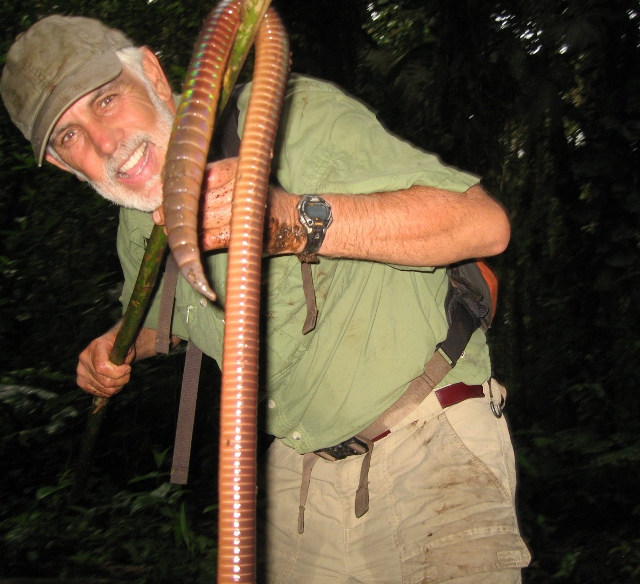
\includegraphics{images/Lab4_giant_worm.png}
\caption{Giant Worm. \url{https://geekologie.com/2014/07/imagine-the-fish-we-could-catch-massive.php}}
\end{figure}

\textbf{Earthworm Life Cycle}

\begin{figure}
\centering
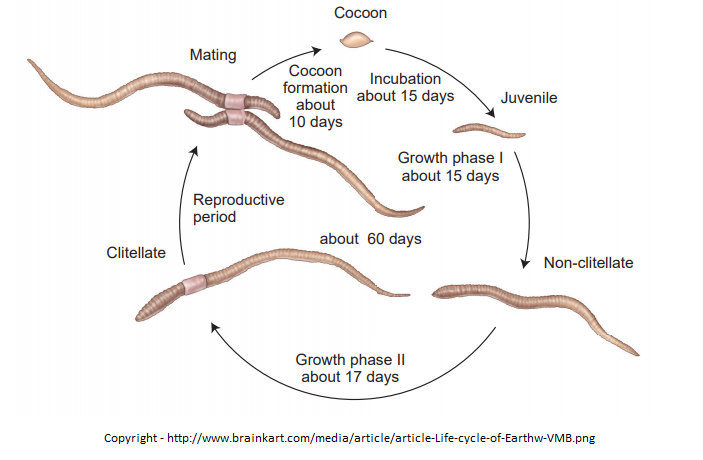
\includegraphics{images/Lab4_earthworm_life_cycle.png}
\caption{Earthworm Life Cycle}
\end{figure}

\textbf{Earthworm Dissection Guide \& Video}

Click \href{https://osf.io/download/tz3uh}{here} to download a copy of the Earthworm Dissection Guide.

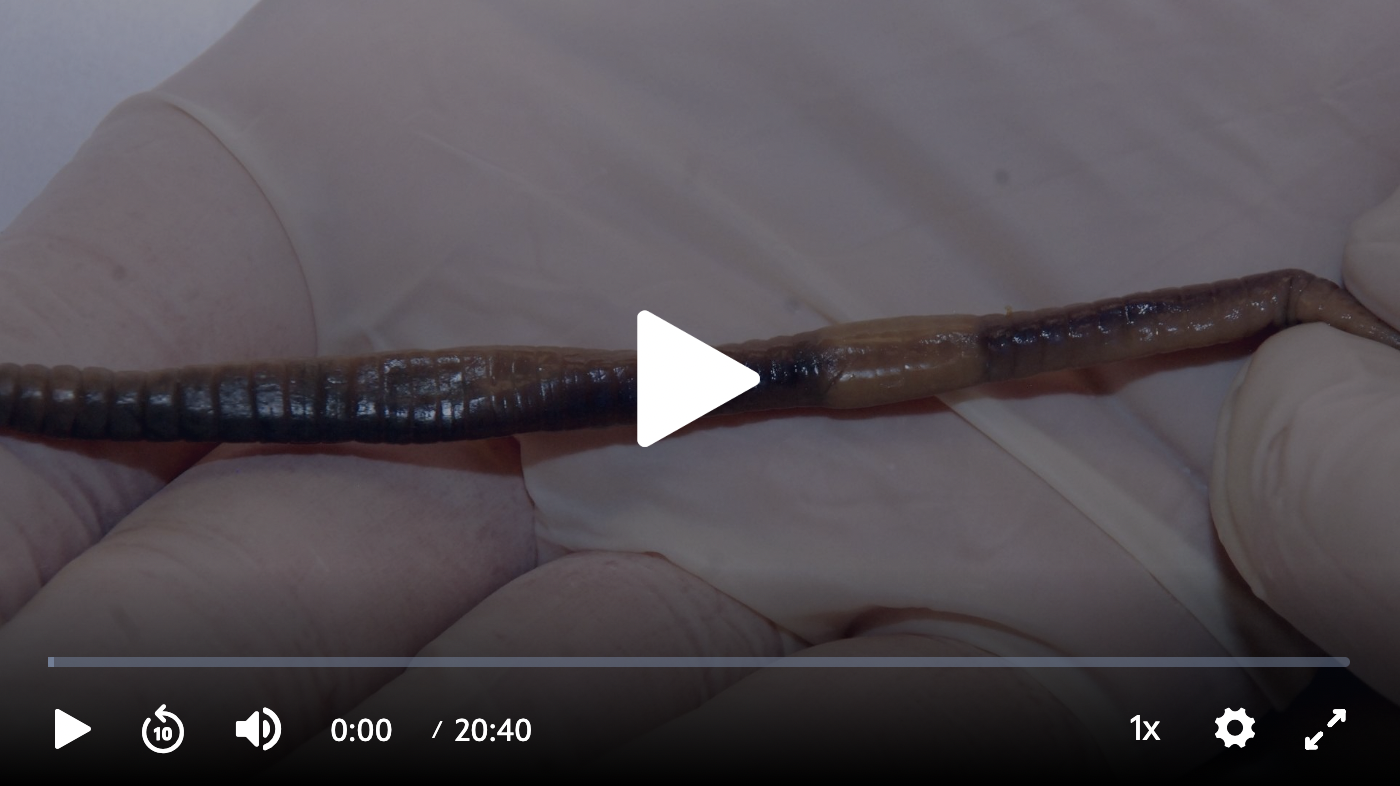
\includegraphics{images/Lab4_Earthworm_Dissection_Video.png}

\textbf{Earthworm Quiz}

Complete the Earthworm Quiz on \href{https://canvas.ubc.ca/}{Canvas}.

\hypertarget{phylum-mollusca-1}{%
\subsection*{Phylum Mollusca}\label{phylum-mollusca-1}}
\addcontentsline{toc}{subsection}{Phylum Mollusca}

Interesting fact: The giant clam has a lifespan well over that of a human!

\begin{figure}
\centering
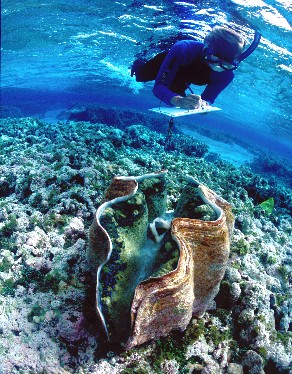
\includegraphics{images/Lab4_giant_clam.png}
\caption{Giant Clam}
\end{figure}

\textbf{Clam Life Cycle}

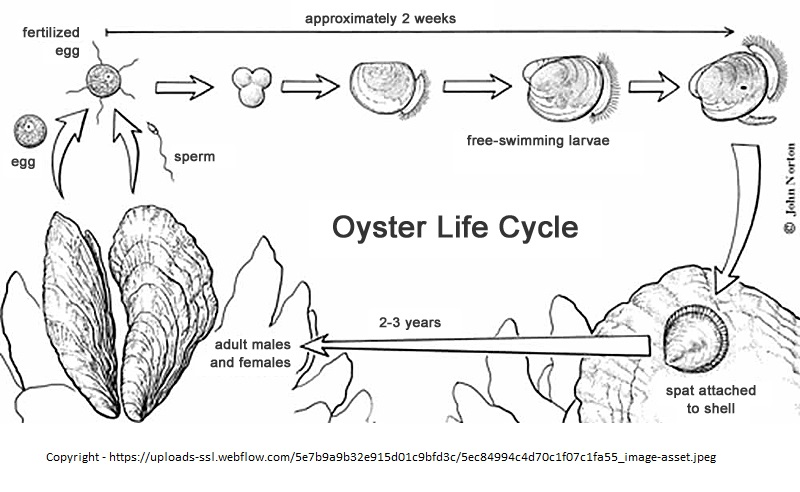
\includegraphics{images/Lab4_clam_life_cycle.png}
\textbf{Clam Dissection Guide \& Video}

Click \href{https://osf.io/download/fevh6}{here} to download a copy of the Clam Dissection Guide.

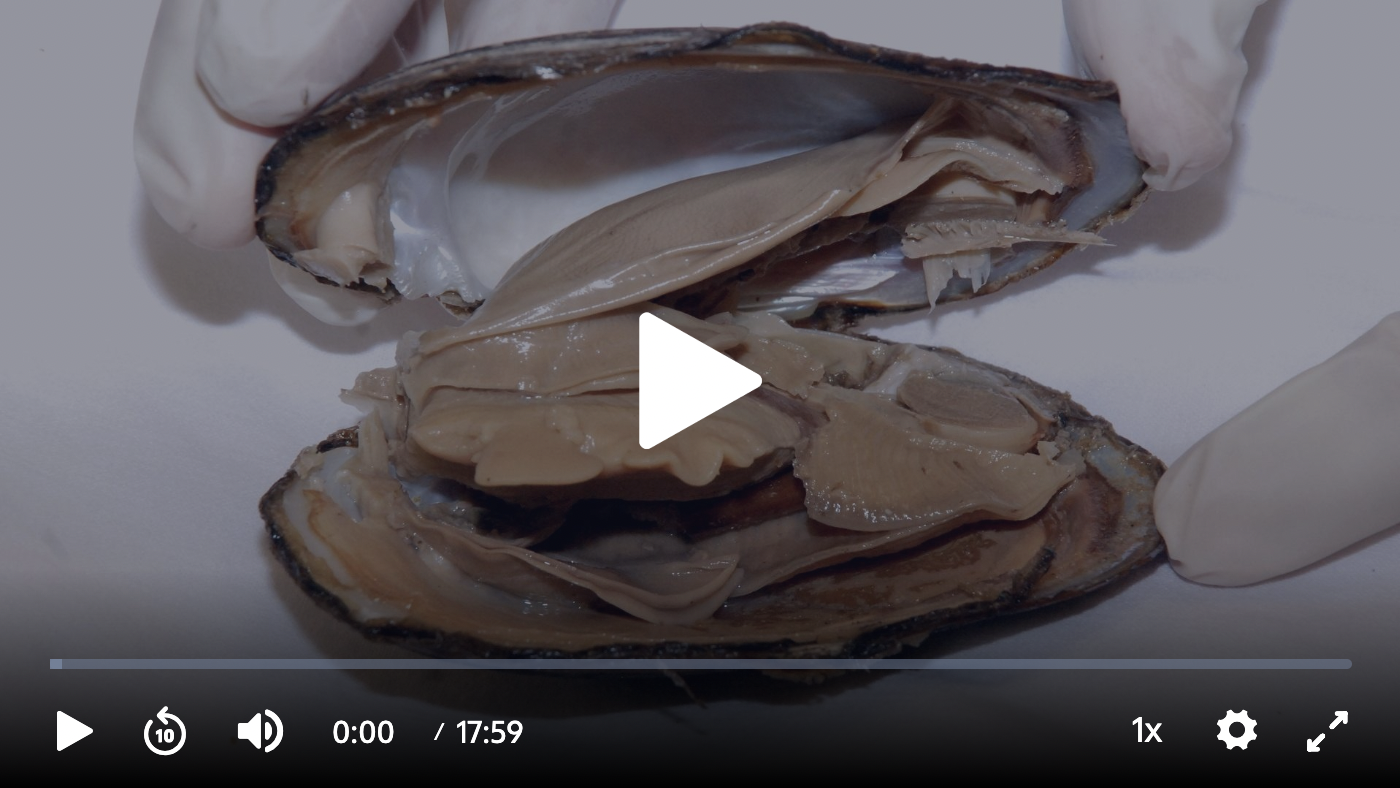
\includegraphics{images/Lab4_Clam_Dissection_Video.png}

\textbf{Clam Quiz}

Complete the Clam Quiz on \href{https://canvas.ubc.ca/}{Canvas}.

\hypertarget{phylum-arthropoda-1}{%
\subsection*{Phylum Arthropoda}\label{phylum-arthropoda-1}}
\addcontentsline{toc}{subsection}{Phylum Arthropoda}

Grasshoppers can make music without any instruments. Click \href{https://www.youtube.com/watch?v=nyglT-rWE5c}{here} to listen to their song.

\textbf{Grasshopper Life Cycle}

\begin{figure}
\centering
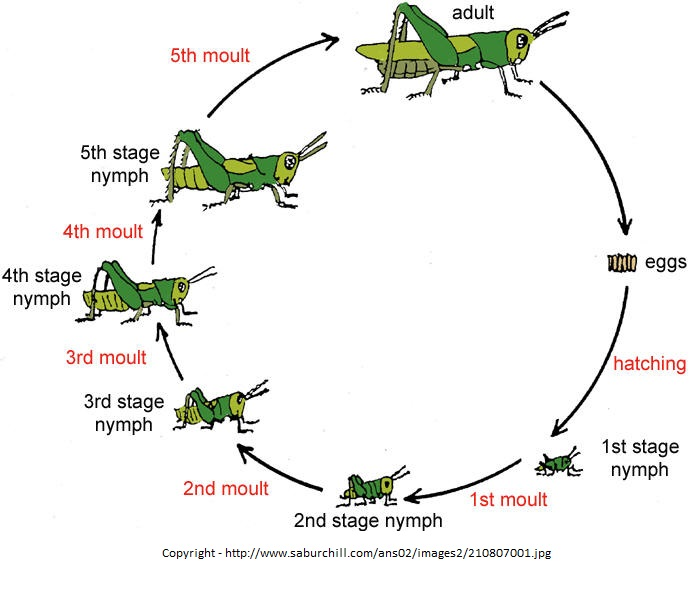
\includegraphics{images/Lab4_grass_hopper_life_cycle.png}
\caption{Grasshopper Life Cycle}
\end{figure}

\textbf{Grasshopper Dissection Guide \& Videos}

Click \href{https://osf.io/download/nk6ub}{here} to download a copy of the Grasshopper Dissection Guide.

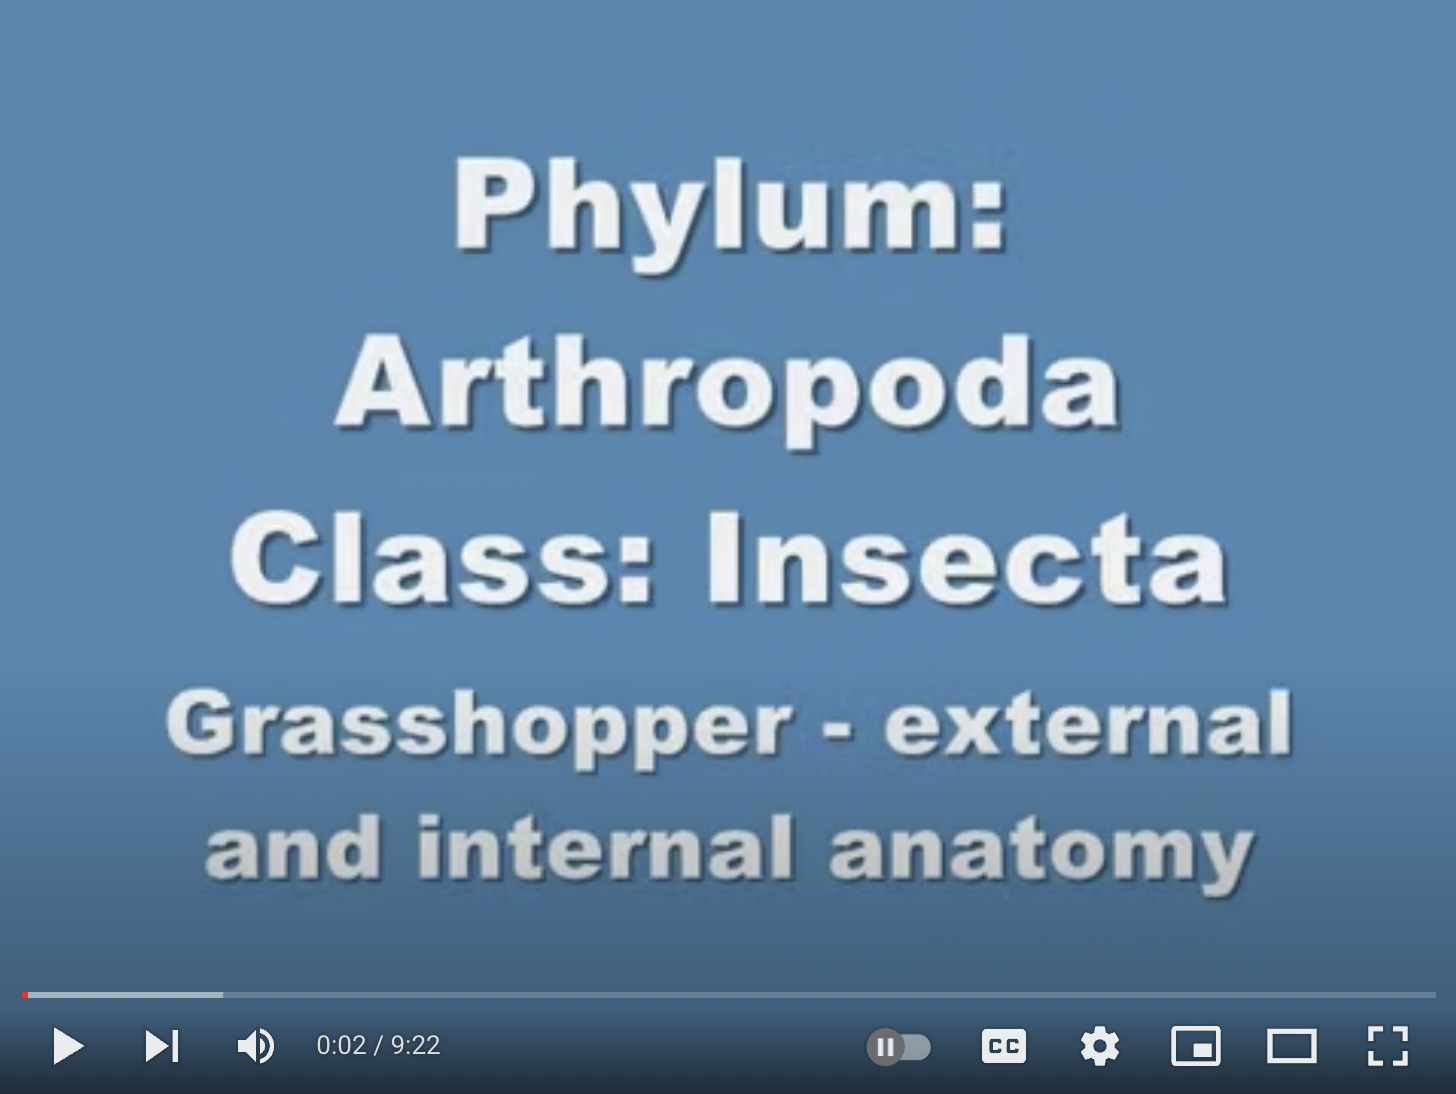
\includegraphics{images/Lab4_Grasshopper_Dissection_Video1.png}

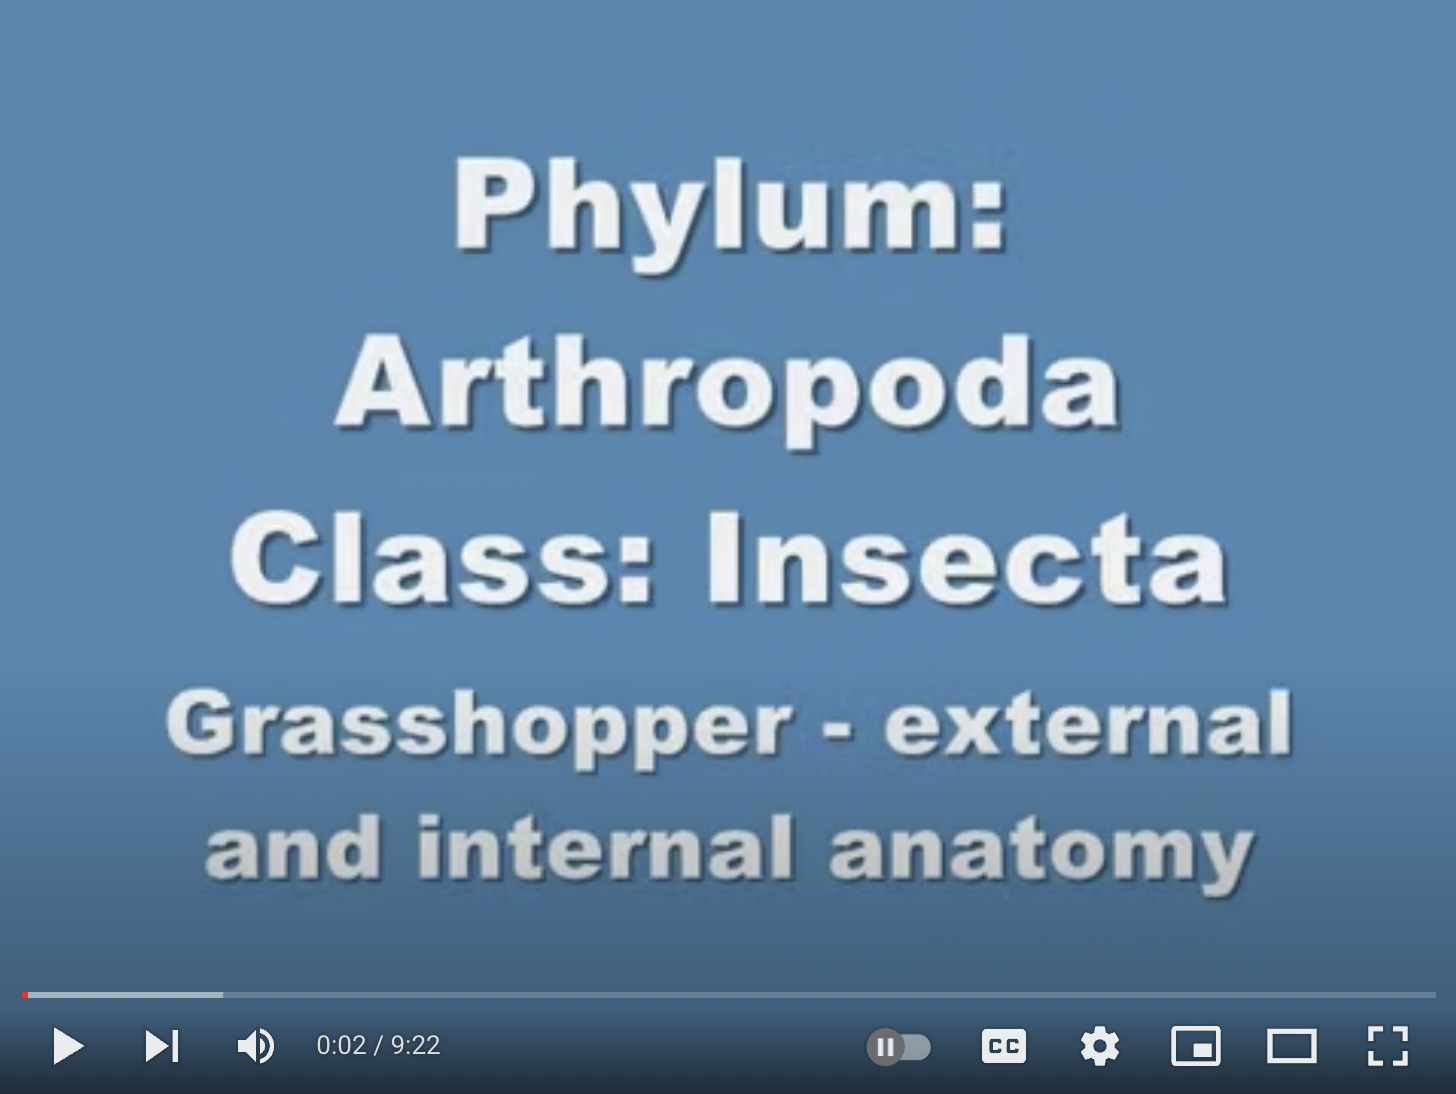
\includegraphics{images/Lab4_Grasshopper_Dissection_Video1.png}

\textbf{Grasshopper Quiz}

Complete the Grasshopper Quiz on
\href{https://canvas.ubc.ca/}{Canvas}.

\hypertarget{assignment-recommendation-report}{%
\chapter*{Assignment: Recommendation Report}\label{assignment-recommendation-report}}
\addcontentsline{toc}{chapter}{Assignment: Recommendation Report}

\href{https://ubco-biology.github.io/Procedures-and-Guidelines/readme-files-and-data-dictionaries.html\#markdown}{In lab 1 you were introduced to Markdown} in the context of documenting your project with \texttt{readmes} and \texttt{data-dictionaries}.

The basic syntax used in Markdown can be found in the \href{https://ubco-biology.github.io/Procedures-and-Guidelines/markdown-1.html}{BIOL Procedures and Guidelines}. In the Procedures and Guidelines you are introduced to generic text editors for writing Markdown.

Markdown is a powerful authoring tool. Part of what makes it powerful is it's integration with other tools, such as \texttt{R}. in BIOL202 you will be introduced to statistical analyses using \texttt{R}. You will also be asked to author reports using \texttt{R} and RMarkdown - \href{https://ubco-biology.github.io/Procedures-and-Guidelines/markdown-flavours.html}{RMarkdown is one flavour of Markdown}. Remember, the content that you're reading right now is all authored using \texttt{R} - when there's analyses being presented - and RMarkdown.

For this assignment, you will be learning RMarkdown and the environment in which we author \texttt{R} and RMarkdown documents - RStudio. You will not be expected to do your analysis in \texttt{R}.

Your Recommendation Report Draft will be submitted as both an RMarkdown document and a pdf. You will also need to include a copy of your data in long format saved as \texttt{.csv} and a \texttt{\_DATA-DICTIONARY.md} file. More details on this in the following sections.

While your Recommendation Report Draft should be approximately 5 double-spaced pages, Times New Roman and font size 12, if you're using RStudio and the templates provided in this class, you should only have to concern yourself with the length of your report; the rest of the formatting will be handled when you export from RMarkdown to pdf.

\hypertarget{science-writing}{%
\section*{Science writing}\label{science-writing}}
\addcontentsline{toc}{section}{Science writing}

Technical science writing is an art. Unlike English style writing, technical science is clear-cut and lacking in artistic enhancements.

Do not quote your sources but rather read through the information and write it in your own words and cite it. It is a good idea to read an article once all the way through without making any notes. Then come back and read it again this time making notes in the margins or on some scrap paper. This will help ensure you not only understand the material you are reading but that you are able to describe it in your own words and avoid issues of plagiarism which so often become in issue for students.

You may wish to review the BIOL Procedures and Guidelins content on \href{https://ubco-biology.github.io/Procedures-and-Guidelines/apa-citations.html}{APA Citations} and \href{https://ubco-biology.github.io/Procedures-and-Guidelines/academic-integrity.html}{Academic Integrity}.

\hypertarget{preparing-to-write}{%
\section*{Preparing to write}\label{preparing-to-write}}
\addcontentsline{toc}{section}{Preparing to write}

Read a lot! It is important that you have a thorough understanding of the topic. At the very least you should have at least 3 primary source papers you are referring too throughout your report to provide further credibility to your recommendation.

Start writing early! Students often make the mistake of starting the night before the lab report is due. This more often than not results in poor submissions and thus lower grades. You should expect that you will have at least 3 rounds of revisions before you submit.

Someone reading your report should be able to tell what question(s) you addressed, why the topic is important, how you tackled the problem, the types of data you will collect, and how your research helps to inform your client.

Need help?

Book an appointment with the the \href{https://students.ok.ubc.ca/academic-success/learning-hub/writing-language/}{Student Learning Hub's writing consultants}!

\hypertarget{a-good-report}{%
\section*{A good report}\label{a-good-report}}
\addcontentsline{toc}{section}{A good report}

A good report includes the following headings / sections

\begin{itemize}
\tightlist
\item
  Abstract
\item
  Data availability statement
\item
  Introduction
\item
  Methods
\item
  Results
\item
  Discussion / Conclusion / Recommendations
\item
  References
\end{itemize}

The goal is to clearly describe to Farmer Elliot what your question was, how you went about answering it, what your results told you and what recommendations you have to help Farmer Elliot make his decision.

\hypertarget{abstract}{%
\subsection*{Abstract}\label{abstract}}
\addcontentsline{toc}{subsection}{Abstract}

An abstract is a brief summary of what the report is all about.

Abstracts in the sciences are approached in a couple of different ways, depending on the sub-discipline and journal preferences. For BIOL125, your abstract should be a single paragraph and no more than 250 words. It should clearly outline the question or problem your research is investigating, describe how the question or problem was addressed and identify the key results and recommendations.

In less than 250 words, the reader should be able to attain the most crucial aspects of each segment of the report within this one paragraph.

\hypertarget{data-availablity-statement}{%
\subsection*{Data availablity statement}\label{data-availablity-statement}}
\addcontentsline{toc}{subsection}{Data availablity statement}

As we learned in BIOL116, when appropriate and feasible, the data underlying our analyses should be made available. You will be asked to submit a \texttt{.csv} file of your data in long format. You may wish to review the content from BIOL116 on \href{https://ubco-biology.github.io/BIOL-116-Lab-Manual/preparing-your-data.html}{Preparing Your Data} and the content on \href{https://ubco-biology.github.io/Procedures-and-Guidelines/tidy-data.html}{Tidy Data} from the BIOL Procedures and Guidelines. You will also be asked to submit a \texttt{\_DATA-DICTIONARY.md} file describing your data. Refer back to the \href{https://ubco-biology.github.io/Procedures-and-Guidelines/data-dictionary.html}{Data Dictionary} section of the BIOL Procedures and Guildelines for guidance and an example.

This is a short statement that indicates if data is available and if it is, how it can be acquired.

\hypertarget{introduction}{%
\subsection*{Introduction}\label{introduction}}
\addcontentsline{toc}{subsection}{Introduction}

\textasciitilde{} 1 page

The introduction should begin with the general topic and then narrow the focus of the details pertinent to the research.

Your introduction should discuss what is currently understood about the topic and how this ties into the study. This is where you want to get across the interesting points of the field that led you to develop your hypothesis and your experimental design. You want to use many sources, particularly primary sources such as journal articles. Ensure your information is cited appropriately (see guidance in the \href{https://ubco-biology.github.io/Procedures-and-Guidelines/apa-citations.html}{BIOL Procedures and Guidelines}). You should have a clear hypothesis stated at the end of this section. This section will be the lengthiest section of your report. Ensure you reader has no doubt where the source of your information comes from.

Your introduction should situate, explain, and identify your research project. It should do this by providing relevant background information that frames the current project and is directly relevant. It should then identify the importance of this particular project. And finally it should clearly articulate the research question and hypothesis being addressed.

\hypertarget{methods}{%
\subsection*{Methods}\label{methods}}
\addcontentsline{toc}{subsection}{Methods}

\textasciitilde{} 1/2 - 1 page

This section of your report involves producing a written description of the materials used and the methods involved in performing your experiment. Under no circumstances should you provide bullet points or list one by one the materials used. Rather you need to describe each step clearly enough that someone else could replicate your experiment exactly. You should also include a section outlining what statistical measure(s) you used and how you transformed your data if need be.

It is highly recommended you show this to someone not in your class and see if they can follow along. If they can't you need to ask them where they get stuck and re-write to make sure it's clear. Think of this like following a recipe while cooking. Don't leave anything out that isn't obvious or the recipe will fail for the next person trying to cook.

Remember, for transparency and reproducibility, your methods are key to your audience understanding how you did exactly what you did. And if you wrote a protocol, it is the methods section against which that protocol will be screened to identify bias.

So, it should be clear, concise, and contain sufficient information for someone else to reproduce the experiment. This means it should include things like, how specimens were procured, how data was collected (tools, measurements etc), and how the data was analysed.

The steps should flow logically, and, while being concise, you should not use bullet points.

\hypertarget{results}{%
\subsection*{Results}\label{results}}
\addcontentsline{toc}{subsection}{Results}

\textasciitilde{} 1/2 - 1 page

The results section is where you will describe what you saw. That is, what the response was to your variable. This should be the driest and easiest section to write as you are just stating what you found and nothing more. There should be no mention of what you did to attain this data or how you went about doing it - that's for your methods section. This is not where you describe why you saw what you saw - that's for your discussion and recommendations section. Nor is it where you try and tie in other research to your research - that's for your introduction and discussion sections.

The results section should include all averaged data from observations during your experiment. This includes charts, tables, graphs, and any other illustrations of data you feel best represents the information you would like to convey. It should not include any raw data. Raw data should be attached as a separate file.

Depending on the information you wish to convey you may feel that a box plot, bar graph or line graph is most descriptive. Whichever way you decide think about what message you are trying to convey and ask yourself if an audience was to quickly look at your graph would they get that messaging easily. If not, you should look at an alternative way to display your graph. Your TA will be able to help you sort this out as well.

Be sure to provide all labels, legends and axes where necessary and a caption which informs the reader of what they are looking at. Remember anyone who is not familiar with your research should be able to quickly look at your figure and understand what message you are trying to show. Please review the BIOL Procedures and Guidelines section on \href{https://ubco-biology.github.io/Procedures-and-Guidelines/figures-tables.html}{Figures \& Tables}.

Your results section should clearly outline the relevant findings from your study and should flow directly from your research question and hypothesis.

This section should include graphs or figures to highlight key findings. Graphs and figures should be present immediately following paragraphs describing the results described by these graphs and figures.

While summary data should be provided, raw data should be not; raw data should be included as supplementary content.

\hypertarget{discussion-conclusions-recommendations}{%
\subsection*{Discussion, Conclusions \& Recommendations}\label{discussion-conclusions-recommendations}}
\addcontentsline{toc}{subsection}{Discussion, Conclusions \& Recommendations}

\textasciitilde{} 1 page

This section is where you will discuss what you saw. Were you able to answer the question you set out to answer? Why or why not? In either case try and explain and interpret your results.

This is where you will want to go back to the journals you found and see what they found. Is it similar or not? Why or why not? Did they do something different from you? You can often explain results you may not have anticipated seeing by looking at what others in the area have found. Think about the why?

Is this the right property for Farmer Elliot or should he keep looking?

Your job here is to try and explain what you found and how it relates to what others have found. From here you will make your recommendation to your client.

\hypertarget{references}{%
\subsection*{References}\label{references}}
\addcontentsline{toc}{subsection}{References}

All references used should be included at the end of your report on a separate page. That includes any books, articles, lab manuals, etc. that you used when writing your report. APA citations are required. Ensure you provide a properly formatted list with sufficient references. At least 3 primary source papers should be listed.

For formatting guidance, refer to the \href{https://ubco-biology.github.io/Procedures-and-Guidelines/apa-citations.html}{APA section} of the BIOL Procedures and Guidelines.

\hypertarget{rmarkdown-and-rstudio}{%
\section*{RMarkdown and RStudio}\label{rmarkdown-and-rstudio}}
\addcontentsline{toc}{section}{RMarkdown and RStudio}

When you're writing \texttt{readme} files and \texttt{data-dictionaries} - or even taking notes in class - a text editor like VS Code is extremely convenient and versatile. When it comes to authoring reports, however, we're going to move you into RStudio.

RStudio is an IDE - an Integrated Development Environment - for \texttt{R}. This is just a fancy way of saying that it's an application that helps you write \texttt{R} code. In BIOL202 and BIOL228, you'll start using RStudio to do analyses in \texttt{R}. Right now, we're just using RStudio to write in RMarkdown and to get used to using the RStudio environment. Along the way, we'll see some \texttt{R} code as we get things set up.

Since RStudio is designed for working with \texttt{R}, we need to install both \texttt{R} and Rstudio. So let's do this.

If you're running a Chromebook, using a tablet, or don't want to install anything new on your computer, all of the Windows computers in the library have \texttt{R} and RStudio installed on them.

While the \texttt{tinytex} package is installed on these machines, it's not loaded out of the box. So, you will need to run the following code in the console

\begin{verbatim}
tinytex::install_tinytex()
\end{verbatim}

If prompted to update the \texttt{rmarkdown} package, do so. There are more details on \texttt{tinytex} and \texttt{rmarkdown} in the 'Getting set up' section below.

\hypertarget{installing-r}{%
\subsection*{\texorpdfstring{Installing \texttt{R}}{Installing R}}\label{installing-r}}
\addcontentsline{toc}{subsection}{Installing \texttt{R}}

\texttt{R} is available from CRAN - the Comprehensive R Archive Network - and is available for all operating systems. Find and download the installer for your operating system at \url{https://cran.r-project.org/}. At the time of writing, the latest version is 4.1.2 Any version that is 4.x.x should be fine for what we'll be doing.


\includegraphics{images/Install-R_20220101.png}

\hypertarget{installing-rstudio}{%
\subsection*{Installing RStudio}\label{installing-rstudio}}
\addcontentsline{toc}{subsection}{Installing RStudio}

Once you have \texttt{R} installed, you can go ahead and install RStudio, also available for all operating systems. Find and download the installer for your operating system at \url{https://www.rstudio.com/products/rstudio/download/\#download}. At the time of writing, the latest version is 2021.09.0+351 This or any later version that is published should be fine for what we'll be doing.

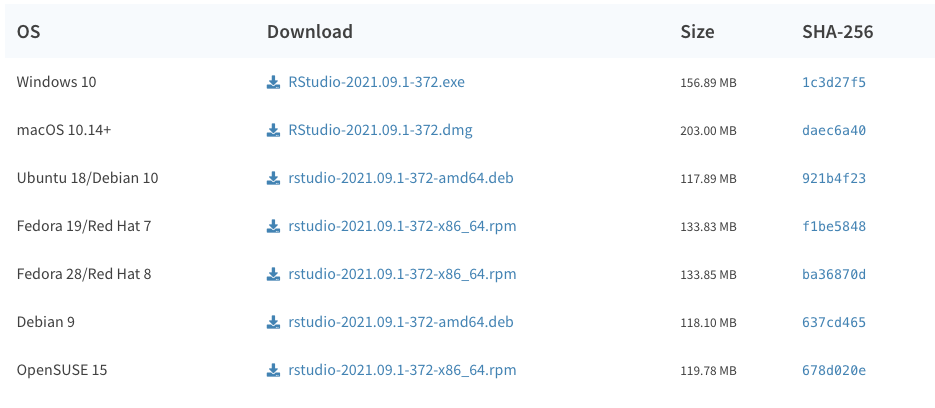
\includegraphics{images/Install-RStudio_20220101.png}

\hypertarget{a-quick-intro-to-rstudio}{%
\subsection*{A quick intro to RStudio}\label{a-quick-intro-to-rstudio}}
\addcontentsline{toc}{subsection}{A quick intro to RStudio}

Your RStudio window is comprised of 4 panes.

\begin{itemize}
\tightlist
\item
  The upper left is where you'll find your working documents.
\item
  The lower left is your console. It is in the console that we can run \texttt{R} code directly if needed.
\item
  The upper right displays information related to your working environment.
\item
  The lower right is where you'll see any output generated by your \texttt{R} code, like figures, help pages etc. It's also where you'll see a file manager so that you can interact with your files directly from within RStudio.
\end{itemize}

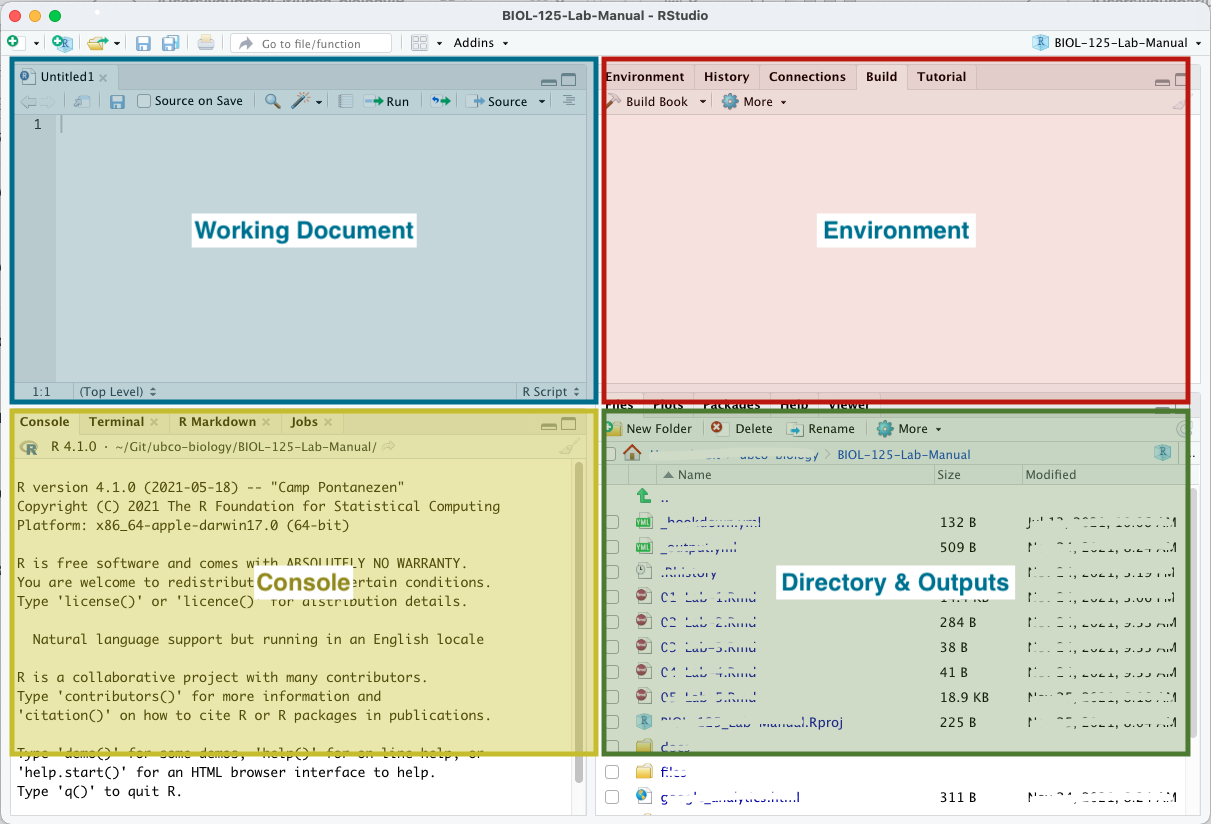
\includegraphics{images/Intro-RStudio_20220101.png}

For report authoring using RMarkdown, we'll mostly be concerned with the upper left pane. We'll occasionally use the console to run a bit of \texttt{R}. And we'll occasionally use the file manager to access files. We won't worry at all about the upper right pane - this will have more relevance when you start computing statistics in \texttt{R} using RStudio.

When you launch RStudio, unless you're opening an existing document, you will only see 3 panes, your console will be on the left, and your environment and output panes will be on the right.

\hypertarget{getting-set-up}{%
\subsection*{Getting set up}\label{getting-set-up}}
\addcontentsline{toc}{subsection}{Getting set up}

Being able to convert from markdown to pdf is not something we can do with the default install of \texttt{R}. We need to get two add-ons to be able to do this. Add-ons in \texttt{R} are called \texttt{packages}. The first package we need to install is \texttt{rmarkdown}. The second is \texttt{tinytex}. \texttt{rmarkdown} handles the general process of reading through your report and getting it ready to be output to a different format. \texttt{tinytex} contains the necessary information to produce a \texttt{pdf}, so \texttt{rmarkdown} will use \texttt{tinytex} for that one part of the conversion process.

The \texttt{x} in \texttt{tinytex} is pronounced like a \texttt{k}, so should read more like \texttt{tinytek} or \texttt{tinytech}.

\hypertarget{installing-rmarkdown}{%
\subsubsection*{\texorpdfstring{Installing \texttt{Rmarkdown}}{Installing Rmarkdown}}\label{installing-rmarkdown}}
\addcontentsline{toc}{subsubsection}{Installing \texttt{Rmarkdown}}

Open RStudio, in the console type the following and hit 'Enter'.

\begin{verbatim}
install.packages("rmarkdown")
\end{verbatim}

You'll see a bunch of stuff written to the console. When it's all done, you'll see your prompt - \texttt{\textgreater{}} - return.

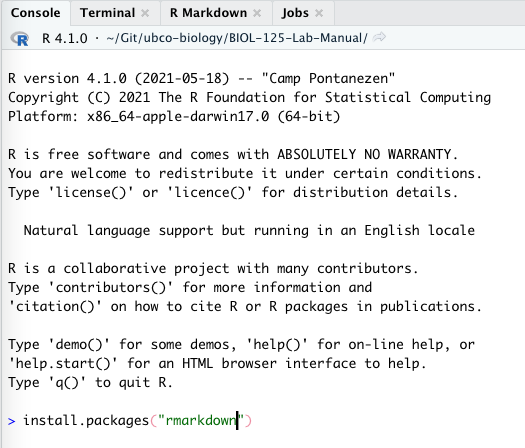
\includegraphics{images/Install-RMarkdown_20220101.png}

\hypertarget{installing-tinytex}{%
\subsubsection*{\texorpdfstring{Installing \texttt{tinytex}}{Installing tinytex}}\label{installing-tinytex}}
\addcontentsline{toc}{subsubsection}{Installing \texttt{tinytex}}

Now, in the console type the following and hit 'Enter' again.

\begin{verbatim}
install.packages("tinytex")
\end{verbatim}

When that's all done, type the following and hit 'Enter'

\begin{verbatim}
tinytex::install_tinytex()
\end{verbatim}

That's it. You should be good to go to open the \texttt{.Rmd} template available in the Assignment tab for this lab.

\hypertarget{recommendation-report-template}{%
\chapter*{Recommendation Report Template}\label{recommendation-report-template}}
\addcontentsline{toc}{chapter}{Recommendation Report Template}

Please use the following template for this assignment:

\href{https://osf.io/download/kcqjs}{20220101\_Lab05\_125\_Assignment\_V1.Rmd} (3 KB)

You will need to submit 4 files for this assignment:

\begin{itemize}
\tightlist
\item
  Recommendation report as \texttt{.Rmd}
\item
  Recommendation report as \texttt{.pdf}
\item
  Data in long, tidy, format as \texttt{.csv}
\item
  Data dictionary as \texttt{.md}
\end{itemize}

You will receive your marked lab report one week from the time it is submitted.

You can decide to resubmit the same lab report draft without making any changes or you will have the opportunity to review the edits and make the needed changes in order to increase your mark.

If you have any questions regarding your mark and / or the comments from your TA please ensure you take the opportunity to chat with your TA to go over these. This will ensure that you are in the best position to attain the highest marks possible for this assignment.

\hypertarget{using-the-template}{%
\subsection*{Using the template}\label{using-the-template}}
\addcontentsline{toc}{subsection}{Using the template}

All the markdown syntax that you need for RMarkdown can be found in the \href{https://ubco-biology.github.io/Procedures-and-Guidelines/markdown-1.html}{Markdown} section of the BIOL Procedures and Guidelines.

\hypertarget{directory-structure-file-naming}{%
\subsection*{Directory structure \& file naming}\label{directory-structure-file-naming}}
\addcontentsline{toc}{subsection}{Directory structure \& file naming}

It is expected that you will have a root project folder for your work associated with this lab. And that at the minimum you will have a folder for your report, your data, and your figures. And that you will download this template into your \texttt{report/} directory. And that lastly, you will rename the template in accordance with the file naming convention you outlined in your first assignment.

This structure and hierarchy will be important when it comes time to include figures and images in your report.

\hypertarget{yaml}{%
\subsection*{YAML}\label{yaml}}
\addcontentsline{toc}{subsection}{YAML}

The top of the template contains some front matter called YAML. YAML provides instructions to all the pieces of software involved in converting your RMarkdown document to it's outputs, in this case, \texttt{pdf}. YAML is very specific to spacing, so don't add any extra spaces!

What you need to do.

\begin{enumerate}
\def\labelenumi{\arabic{enumi}.}
\tightlist
\item
  Provide a title within the quotations after \texttt{title}.
\item
  Provide your name within the quotations after \texttt{author}.
\item
  Provide your abstract within the quotations after \texttt{abstract}.
\end{enumerate}

What might be nice to know.

\begin{enumerate}
\def\labelenumi{\arabic{enumi}.}
\tightlist
\item
  r Sys.Date() pulls the date from your computer and auto populates this for you.
\item
  The \texttt{output} tag defines the output format. Other options include \texttt{html\_document} and \texttt{word\_document}.
\end{enumerate}

What exactly is YAML?

\begin{quote}
YAML™ (rhymes with ``camel'') is a human-friendly, cross language, Unicode based data serialization language designed around the common native data types of dynamic programming languages. It is broadly useful for programming needs ranging from configuration files to internet messaging to object persistence to data auditing and visualization.
\end{quote}

Read more at \href{https://yaml.org/}{the Official YAML Web Site}

\hypertarget{document-body}{%
\subsection*{Document body}\label{document-body}}
\addcontentsline{toc}{subsection}{Document body}

The template is then pre-populated with first level headers for each section you're expected to include in your report. Each heading re-iterates the key elements the content of these headings should address. This is just place holder text, so replace it with your own.

\hypertarget{images-graphs}{%
\subsection*{Images \& graphs}\label{images-graphs}}
\addcontentsline{toc}{subsection}{Images \& graphs}

There is one sample graph included. Note how it references the figure to be included \texttt{../figures/image-name.png} The \texttt{../} means 'go one level up in the directory' which, if you have your project set up in the following way and your \texttt{.Rmd} file is in your \texttt{report/} directory it means 'look in the \texttt{root/} directory for a folder called \texttt{figures/}.

\begin{verbatim}
root/
  report/20220101_Lab05_125_Assignment_V1.Rmd
  data/
  figures/MVD_BIOL125-Lab5_Fig-1-Boxplot_V1.png
\end{verbatim}

If you make a mistake in setting this path, you'll get the following error in RStudio

\begin{verbatim}
(No image at path ...)
\end{verbatim}

You'll also note the following directly after the image path: \texttt{\{width=50\%\}}. This reduces the image size by 50\%. This works well for the images produced by the ShinyApp used in this course.

As noted in the template, you do not need to write \texttt{Figure\ 1:} before your figures; this small piece of text is handled during the conversion from RMarkdown to pdf. Any other information that you would like to include in the caption should go in the \texttt{{[}{]}} before the \texttt{()} that contain the path to the image.

Figure placement

The engine behind the conversion from RMarkdown to pdf is a typesetting application, one with pretty strict rules about how content should be formatted - much more strict than something like Microsoft Word.

What this means is that if the placement of your images will disrupt your prose - by creating large amounts of empty white space for example - this typesetting application will \emph{push} your figure to somewhere lower in your report where it won't create this white space.

Your figures should be adjacent to the relevant text in your RMarkdown file. How this manifests to your pdf might look a little different; that's ok.

\hypertarget{references-1}{%
\subsection*{References}\label{references-1}}
\addcontentsline{toc}{subsection}{References}

Just before the heading for references you'll see the following

\begin{verbatim}
\clearpage
\end{verbatim}

This creates a page break between your references section and the rest of your report.

\hypertarget{building-the-pdf}{%
\subsection*{\texorpdfstring{Building the \texttt{pdf}}{Building the pdf}}\label{building-the-pdf}}
\addcontentsline{toc}{subsection}{Building the \texttt{pdf}}

If you've installed \texttt{R}, RStudio, and the \texttt{markdown} and \texttt{tinytex} packages succesfully, when you open the template \texttt{.Rmd} file you should see an option to \texttt{Knit}.

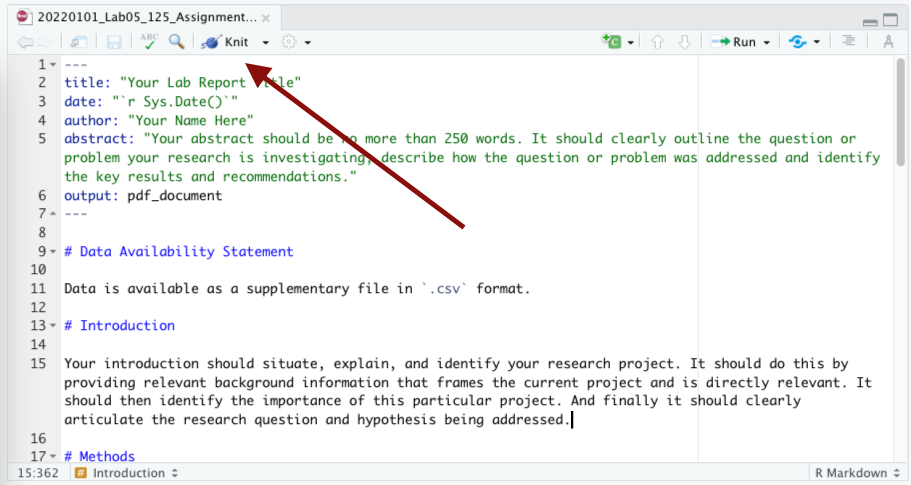
\includegraphics{images/Knit_20220101.png}

Click this button or select the drop down arrow and select \texttt{Knit\ to\ pdf}. This will generate a pdf in the same directory as your \texttt{.Rmd} file.

To test this with the template, ensure the template \texttt{.Rmd} file is in your \texttt{report/} directory and download the following image into your \texttt{figures/} directory

\begin{itemize}
\tightlist
\item
  \href{https://osf.io/download/nrzdu}{MVD\_BIOL125-Lab5\_Fig-1-Boxplot\_V1.png} (4 KB)
\end{itemize}

You should get something that looks like this after \texttt{Knitting} the \texttt{.Rmd} file

\begin{itemize}
\tightlist
\item
  \href{https://osf.io/download/6kn7m}{20220101\_Lab05\_125\_Assignment\_V1.pdf} (180 KB)
\end{itemize}

\hypertarget{recommendation-report-rubric-1}{%
\chapter*{Recommendation Report Rubric}\label{recommendation-report-rubric-1}}
\addcontentsline{toc}{chapter}{Recommendation Report Rubric}

\begin{longtable}[]{@{}
  >{\raggedright\arraybackslash}p{(\columnwidth - 4\tabcolsep) * \real{0.3333}}
  >{\raggedright\arraybackslash}p{(\columnwidth - 4\tabcolsep) * \real{0.3333}}
  >{\raggedleft\arraybackslash}p{(\columnwidth - 4\tabcolsep) * \real{0.3333}}@{}}
\toprule()
\begin{minipage}[b]{\linewidth}\raggedright
Criteria
\end{minipage} & \begin{minipage}[b]{\linewidth}\raggedright
Description
\end{minipage} & \begin{minipage}[b]{\linewidth}\raggedleft
Pts
\end{minipage} \\
\midrule()
\endhead
Abstract & Brief, no more than 250 words. Clearly outlines the question / problem. Clearly describes how the question/problem was addressed. Results and recommendations are provided. & 4 \\
Data Availability & Data availability statement is present. & 1 \\
Introduction & Relevant background information provided. Clearly articulates how the background information is connected to the current project. Importance of this project has been described. Written well and easy to follow. Flows from more general and broad background information to the focus of the project. Hypothesis and questions posed are outlined at the end of this section. No factual errors are present. & 7 \\
Methods & No bullet points. All methods and materials are clearly described. Easy to follow. Enough information has been provided for others to be able to reproduce the experiment. Data analysis procedure is also included. & 4 \\
Experimental Design & Procedure is specific and addresses the question / problem. Data collection is clearly defined. Appropriate control (where applicable) has been used. Independent and dependent variables are identified. Student testing only one variable. & 5 \\
Results & Includes graphs / figures. No raw data is provided outside of supplemental. Clearly outlines the findings from the study. Flow is sensible with figures present immediately following paragraphs describing the results of figure. & 4 \\
Figures & Are present. Figure selected is best for this type of data. All axes are labelled with units present where applicable and legends found. All figure present have been discussed in write up. Only averages are being shown. Appropriate statistical measures are present. Figures are clear and easy to interpret. No figures present without being discussed. & 7 \\
Discussion \& Recommendation & Student displays clear understanding of results. Student displays a clear understanding of the meaning of these results. Interpretation of results is founded in the data, observations and/or other studies. Recommendations are sound and based on the current study and / or other studies. & 4 \\
Spelling \& Grammar & No spelling errors. No grammar errors. No awkward sentence structures. & 3 \\
References \& in-text citations & APA format used properly and consistently. Minimum of 3 primary source papers used in the report. In-text citations are used when required. Citations and references match up. & 4 \\
Plagiarism \& Quotations & No plagiarism of any kind has been found. No quotations present. Information attained from outside resources are properly cited. & 3 \\
File Uploads \& Format & A total of 4 files have been submitted. Report has been submitted as \texttt{pdf} and RMarkdown. Report is no more than 5 pages (excluding references). Data has been submitted in Tidy format as \texttt{csv}. Data dictionary has been submitted as \texttt{.md}. & 4 \\
\textbf{Total} & & \textbf{50} \\
\bottomrule()
\end{longtable}

Your Recommendation Report Draft is due this week. Submit your draft \textbf{before 11:59 pm on July 18th} to avoid a late penalty or a zero!

\hypertarget{part-lab-5}{%
\part*{Lab 5}\label{part-lab-5}}
\addcontentsline{toc}{part}{Lab 5}

\hypertarget{animal-systems-i-part-two}{%
\chapter*{Animal Systems I: Part Two}\label{animal-systems-i-part-two}}
\addcontentsline{toc}{chapter}{Animal Systems I: Part Two}

\emph{Last updated 2022-08-22}

\hypertarget{overview-of-the-week-1}{%
\subsection*{Overview of the Week}\label{overview-of-the-week-1}}
\addcontentsline{toc}{subsection}{Overview of the Week}

Breakdown:

\begin{enumerate}
\def\labelenumi{\arabic{enumi}.}
\tightlist
\item
  Come to lab ready on campus
\item
  Get assigned an animal and a group by your TA
\item
  Build a quiz for your fellow students in the lab
\item
  Complete two quizzes written by your fellow students in the lab
\item
  Submit Assignment \#4 before the end of the lab. Ensure all members have submitted a copy or those students missing a submission will receive a zero for the assignment and an absence score of 2.5.
\end{enumerate}

Last lab you spent a tremendous amount of time learning about annelids, molluscs, and arthropods through videos, images, guides, and quizzes. Now, this week you will get to see these animals up close and personal!

For this week, you will be placed in groups and will be performing some dissections! Though not required, if you have lab coats please feel free to bring them along. All needed gloves and eye protection will be provided in the lab. For those of you who are not comfortable with dissections please know that you can still participate in the activity without having to do the actual dissection.

Make notes and work together as a team to learn, not only about the animal you will be assigned but also those of the other groups, and make a quiz to test other students' knowledge about your animal. Your TA will provide more details about the logistics of how this will work in the lab. In either case, have fun and enjoy the process!

\hypertarget{assignment-lab-5}{%
\chapter*{Assignment: Lab 5}\label{assignment-lab-5}}
\addcontentsline{toc}{chapter}{Assignment: Lab 5}

Click \href{https://osf.io/download/rh8nv}{here} to download a copy of Assignment 4.

\hypertarget{part-lab-6}{%
\part*{Lab 6}\label{part-lab-6}}
\addcontentsline{toc}{part}{Lab 6}

\hypertarget{animal-systems-ii-part-one}{%
\chapter*{Animal Systems II: Part One}\label{animal-systems-ii-part-one}}
\addcontentsline{toc}{chapter}{Animal Systems II: Part One}

\emph{Last updated 2022-08-22}

\hypertarget{overview-of-the-week-2}{%
\subsection*{Overview of the Week}\label{overview-of-the-week-2}}
\addcontentsline{toc}{subsection}{Overview of the Week}

\begin{enumerate}
\def\labelenumi{\arabic{enumi}.}
\tightlist
\item
  You will be joining your lab mates and TA during your regular scheduled time but online
\item
  Your TA will go through a PowerPoint presentation online
\item
  You will be given time to review all material provided on Canvas
\item
  You must complete all quizzes for this week's lab provided on Canvas due \textbf{before 11:59 pm on July 25th}
\item
  Submit your final recommendation report Assignment \#3 \textbf{before 11:59pm on July 28th}
\end{enumerate}

This week you will be working your way through the material posted on Canvas online but during your scheduled lab time. Your TA will spend time going over a quick \href{https://osf.io/download/cf6tb}{PowerPoint presentation} regarding these animals. You will then need to spend a fair bit of time going through the different videos, images, and written material provided to ensure you have a solid grasp of these animals before coming to campus next week for your synchronous week. You must complete all quizzes associated with the animals found in animal systems II \textbf{before 11:59 pm on July 27th}. Even though you will be getting together this week there is no reason you can't start reviewing all this information ahead of time so that you are better prepared to get through the material during your lab section.

\hypertarget{animal-systems-information-ii}{%
\chapter*{Animal Systems Information II}\label{animal-systems-information-ii}}
\addcontentsline{toc}{chapter}{Animal Systems Information II}

\hypertarget{phylum-echinodermata}{%
\subsection*{Phylum Echinodermata}\label{phylum-echinodermata}}
\addcontentsline{toc}{subsection}{Phylum Echinodermata}

\emph{Biology 125 Biology for Science Majors II Lab Manual. Written by Dr.~Tristyn Hay October, 2021. Some content provided by the University of British Columbia and Okanagan Biology Graduate Program students handbook The Fictional Animal Project: A Tool for Helping Students Integrate Body Systems. Adv. Physiol. Edu 41: 239-243 Blatch et al.~2017}

A ``spiny skin'' characterizes members of the phylum Echinodermata, by only living in marine environments, and by possessing a unique water vascular system. The are also radially symmetrical as adults, but not as larvae. The spiny skin is actually an endoskeleton made up of calcareous plates. Typical echinoderms include seastars (starfish), brittle stars, sea urchins, sand dollars, sea cucumbers and sea lilies. According to DNA evidence, they are closely related to members of the Phylum Chordata, the phylum to which humans belong. Chordates andechinoderms also share a similar pattern of embryonic development, as both are deuterostomes.

\textbf{EXTERNAL FEATURES OF THE SEASTAR}

Pisaster can be seen in the crevices of intertidal rocks and covering the pilings of piers and docks. Pisaster is a rapacious predator on bivalves, but little eats it, except for the occasional desperate seagull.

The underside of the seastar is referred to as the oral side; the opposite side is the aboral side. The external features on the aboral side include the rays (arms) and sieve plate (madreporite). On the surface there are small calcareous bumps called spines and between them arestructures called dermal papillae (not visible with the naked eye). On the mouth side tube feet, the mouth and ambulacral groove can be observed.

The sea star uses its water vascular system to capture food and in locomotion and respiration. Water enters the system via the sieve plate. The water is then moved along through a series of canals by the action of cilia out to the rays and to the ampullae. Contraction of an ampulla forces water into a tube foot lengthening it. Contraction of longitudinal muscles in the foot forces water back into the ampulla shortening the foot. Small suction discs at the end of the feet allow the starfish to move on hard ground and to grasp its prey. The tube feet are also important sites of gas exchange. Pressure generated by the water vascular system also allows the seastar to evert its cardiac stomach and pry open the shells of bivalves like clams, in order to eat them. It is important to realize that the water vascular system is not a true a vascular system supplied with a heart as a pump, and that there is no blood that contains special pigments for transporting gases (as is seen in other animals with true vascular systems). \href{http://www.youtube.com/watch?v=p0VM67cQUWw\&feature=related}{Video of tube feet in action}

\textbf{DIGESTION}

Seastars feed by everting part of the cardiac stomach through their mouths out into the water (or even directly into the shells of molluscs). Then the food is either brought back into the body of the seastar for digestion or digested in place outside the seastar's body. This allows it to feed on animals much larger than itself. Without being able to evert one of its stomachs, the hard endoskeleton would limit the size of prey that could be eaten by the seastar. The cardiac stomach passes the food to the pyloric stomach, where more digestion takes place. Most of the space in the ray is taken up by two highly branched digestive glands (also called pyloric caeca). They secrete digestive juices from their many lobes. They are connected to the pyloric stomach by a pyloric duct in each ray. Absorption of nutrients occurs in the digestive glands.

\textbf{TRANSPORT AND EXCHANGE}

Gas exchange occurs through two types of structures that extend from the surface of the seastar: the tube feet and the papillae (also called papulae or gills); the latter are thin-walled extensions of the body cavity (coelom) that extend onto the aboral surface of the seastar. They look like small finger-like sacs when the animal is in the water, but may not be visible on these specimens. There is no circulatory system in the seastar. Instead, gases are carried around the body via fluids in the body cavity, powered by the action of cilia.

In one ray the digestive glands have been removed to show the ampullae of the tube feet, which are the bulbs on the aboral side of the tube feet, which contract to extend the tube feet.

\textbf{EXCRETION AND OSMOREGULATION}

In seastars, nitrogenous waste is excreted as ammonia. Solid waste is expelled through the anus. There is no osmoregulation in seastars. They are osmoconformers.

\textbf{REPRODUCTION}

Sometimes individual animals are male or female (dioecious). In other cases, the same gonadcan produce both eggs and sperm, either simultaneously or sequentially. External fertilization occurs after the gametes have been released through ducts located on the central body between the arms.

\hypertarget{phylum-chordata-perch}{%
\subsection*{Phylum Chordata-Perch}\label{phylum-chordata-perch}}
\addcontentsline{toc}{subsection}{Phylum Chordata-Perch}

Phylum Chordata includes all those animals (perhaps 50,000 species) with backbones: fish,
amphibians, mammals, reptiles, birds, as well as a few other species. A few chordates do not have backbones and are thus classified as invertebrates. These include small marine animals called tunicates and lancelets. To be a chordate an animal must:

\begin{enumerate}
\def\labelenumi{\arabic{enumi}.}
\tightlist
\item
  Have had at least during embryonic development, a structure called a notochord. (this is a flexible supportive rod running longitudinally through the dorsum of the animal just ventral to the nerve cord; it becomes the spinal column in vertebrates);\\
\item
  have pharyngeal gill slits at some stage in their development;
\item
  have a dorsal hollow nerve cord, and
\item
  Have a post-anal tail.
\end{enumerate}

The perch is a chordate belonging to the Actinopterygii (ray-finned fishes) within the subphylum Vertebrata. Well over 25,000 ray-finned fish species are known today and, as we probe deep ocean regions, we will find many more. Perch are freshwater food and game fish found in Europe
and North America. Perca fluviatilis or yellow perch is a marginal sport fish, which has been introduced into Vaseux and Osoyoos Lakes in the Okanagan.

\textbf{THE PERCH -- EXTERNAL FEATURES}

Be sure that you can identify the dorsal and ventral sides of your specimen and its anterior and
posterior ends. Be able to draw and identify the pectoral, dorsal, pelvic, anal, and caudal fins.\\
Most fish have external fertilization, but a few species, like guppies, have internal fertilization and are livebearers.

\textbf{DIGESTION}

Perch are carnivores. Their digestive tract comprises an alimentary canal (the tube running from the mouth to the anus) as well as accessory structures, such as the liver, salivary glands and pancreas. After the mouth, the alimentary canal includes, in order, the esophagus, stomach, pyloric caeca (secretory and digestive functions), intestine and duodenum.

\textbf{CIRCULATION AND RESPIRATION}

Perch, being aquatic chordates, use gills as a respiratory exchange surface. Cut away the bony
operculum to expose the gill chamber and its four gills. Remove an individual gill to study its structure. The hard-bony support is the gill arch, with posteriorly directed gill filaments. The hard-anterior finger-like projections, the gill rakers, prevent coarse material or food from passing through the gill slits. Gill filaments are supplied with capillary beds across which gas exchange occurs. The flow of blood is opposite to the flow of water across the gills, called counter-current flow; this enhances the concentration gradient and thus the rate of diffusion. This helps metabolically active fish to more efficiently extract oxygen from relatively poorly (relative to air) oxygenated water.

Chordates have closed circulatory systems. The advantage of a closed circulatory system over an open system is that blood can be kept at a higher pressure thus moving through the body more quickly, which is more efficient at servicing body tissues.

The pericardial cavity, just beneath and ventral to the gills, contains the two-chambered heart. Observe the thin-walled posterior atrium extending over the thicker-walled ventricle. Anterior to the ventricle is the bulbus arteriosus, the enlarged base of the ventral aorta that carries blood to the gills and on to the rest of the body. The blood is under pressure when it reaches the gills, but pressure is reduced when the blood passes through the capillary bed. Blood pressure remains low as the blood travels to the rest of the body. This is different from animals with a pulmonary loop, in which the blood travels back from the lungs to the heart, where it is pumped (re-pressurized) to the rest of the body and thus can move more quickly and service body tissues more efficiently than the lower pressure system.

\textbf{EXCRETION AND OSMOREGULATION}

Chordates have kidneys composed of nephrons. In fish and amphibians, the kidneys lie as two straps alongside the spinal column; in reptiles they become attenuated to the posterior portion of the animal, and this phenomenon is even more advance in birds and mammals. Kidneys function as both excretory and osmoregulatory organs. In addition, osmoregulation can be facilitated by other organs, depending upon the type of animal.

In freshwater fish like the perch, the kidney excretes large amounts of dilute urine in order to rid the body of excess water. In marine fish, the kidney excretes salt ions in very concentrated urine.
In all fish, ammonium is the form of nitrogenous waste excreted.

\hypertarget{phylum-chordata-rat}{%
\subsection*{Phylum Chordata-Rat}\label{phylum-chordata-rat}}
\addcontentsline{toc}{subsection}{Phylum Chordata-Rat}

Rats are examples of terrestrial chordates. They are also mammals. Therefore, their anatomy will reflect the fact that they get their oxygen from air, must conserve water, and have internal fertilization with their offspring then developing in a uterus before being born.

\textbf{DIGESTION}

As in all tetrapods, the anterior end of the digestive and respiratory systems is shared. Air, water and food all pass through the oral cavity. In the pharynx, the epiglottis acts as a gate to direct air into the lungs and food or water into the rest of alimentary canal. Like in the perch, the digestive
system comprises the alimentary canal (oral cavity, pharynx, esophagus, stomach, small intestine, large intestine, rectum and anus). Each part of the alimentary canal is specialized for a particular function: mechanical or chemical digestion, absorption of water or nutrients, or retention or elimination of undigested solid wastes. Be able to identify the stomach, small intestine, salivary glands, liver, and spleen in preparation for your lab exam.

The accessory structures of the digestive tract include the liver, pancreas and salivary glands. These are exocrine glands, meaning that they secrete chemicals into ducts that lead directly to another structure - in this case, the alimentary canal specifically, the accessory structures supply enzymes, or other chemicals that aid in digestion, to the alimentary canal.

\textbf{CIRCULATION AND REGULATION}

After being directed from the pharynx into the respiratory system, air enters the trachea, the bronchi and then the lungs. The lungs of amphibians are fairly simple invaginated sacs of vascularized epithelial tissue in which there are internal partitions to increase the surface area. Birds and mammals, however, have lungs of a more complex nature. In mammals, the bronchioles divide into finer and finer branches until they end in tiny, blind-ended sacs called alveoli, which greatly increase the surface area across which gas exchange occurs. Birds have
other mechanisms to increase gas exchange.

Because air movement into and out of the lungs is based on differences in air pressure, it is important that the lungs be sealed in an air-tight part of the body where movement of muscles
can create differences in pressure. This area is called the thoracic cavity. Differences in pressure
within the thoracic cavity are created by movement of muscles associated with the ribs, as well as the diaphragm.

The heart of the rat, like all mammals, consists of four chambers: two atria and two ventricles. When the atria contract they fill their respective ventricle with blood; when the ventricles contract, the increased pressure directs blood from the right ventricle to the lungs and from the left ventricle to the rest of the body. Your rat has been double-injected with latex. Blue latex was injected into the veins and red latex was injected into the arteries. Entering the right atrium are three main blood vessels that bring the deoxygenated blood back to the heart from all regions of the body. These blood vessels are the right superior vena cava, the left superior vena cava and the inferior vena cava. The right and left superior venae cavae return deoxygenated blood to the heart from the right and left side of the head, neck and forelimbs. The inferior vena cava returns deoxygenated blood to the heart from the lower part of the body. More in depth detail of a mammal heart will be covered in the next lab.

\textbf{EXCRETION AND OSMOREGULATION}

Rat kidneys, like those of humans, excrete urea. Urea is less toxic than ammonia therefore it requires less water to be excreted; however, energy must be expended in order to make urea from ammonia. Organisms that use urea tend to live in environments where water conservation
is important. Rat kidneys lie outside of the abdominal cavity, behind the lining of connective tissue. Thus, they are said to be retroperitoneal. The kidneys are the major osmoregulatory organ in the rat.

\textbf{REPRODUCTION}

In male rats, the scrotum, a large sac of skin, muscle and connective tissue holds the testes on
the exterior of the body just ventral to the anus. During non-breeding periods, the testes may be retracted into the abdominal cavity and the scrotum will not be enlarged. Around the outside of each testis is a C-shaped structure known as the epididymis, which is a very long, highly coiled
tubule. Part of the epididymis is on the posterior end of the testes and part is on the anterior end. Sperm cells produced in the seminiferous tubules of the testes pass into the epididymis and then into the vas deferens, which is a moderately large tube leading from the epididymis to the urethra, which is a tube located inside the penis. The penis is enclosed in an epithelial sheath and held along the ventral wall of the abdomen.

The prostate glands are found on either side of the urinary bladder. These glands, and some other glands in this region, comprise the accessory sex glands. The secretions of these glands form the seminal fluid, which carries the sperm during ejaculation, activates and provides certain nutrients for them, and contains substances that neutralize the somewhat acid environment in
the vagina.

In female rats, as in all mammals, the eggs are produced in the ovaries and then released into the
oviducts, through which they travel to the uterus. If fertilization occurs, the fetuses develop in the uterus. The rat uterus has two horns, which join at their base to form the vagina.

\hypertarget{life-cycles-dissection-guides-videos-1}{%
\chapter*{Life Cycles, Dissection Guides, \& Videos}\label{life-cycles-dissection-guides-videos-1}}
\addcontentsline{toc}{chapter}{Life Cycles, Dissection Guides, \& Videos}

\hypertarget{phylum-echinodermata-1}{%
\subsection*{Phylum Echinodermata}\label{phylum-echinodermata-1}}
\addcontentsline{toc}{subsection}{Phylum Echinodermata}

Did you know that a seastar eats with its stomach outside itself? Click the video below to see for yourself! \url{https://www.shapeoflife.org/video/echinoderms-sea-star-time-lapse-eating-mussel}

\textbf{Seastar Life Cycle}

\begin{figure}
\centering
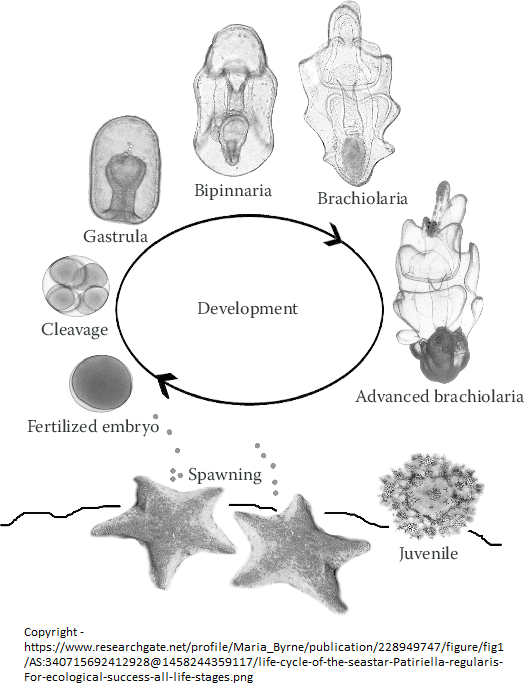
\includegraphics{images/Lab6_seastar_life_cycle.png}
\caption{Seastar Life Cycle}
\end{figure}

\textbf{Seastar Dissection Guide \& Video}

Click \href{https://osf.io/download/y89wz}{here} to download a copy of the Seastar Dissection Guide.

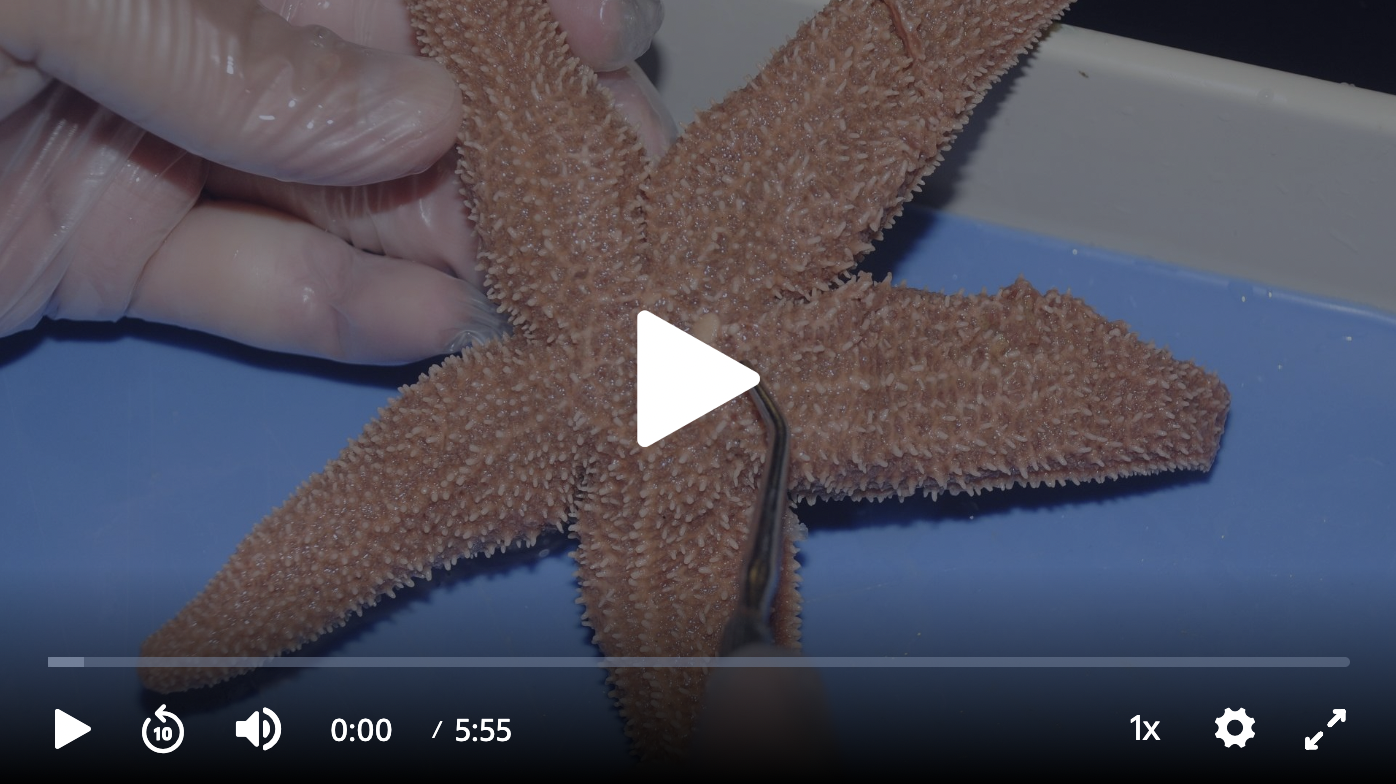
\includegraphics{images/Lab6_Seastar_Dissection_Video1.png}

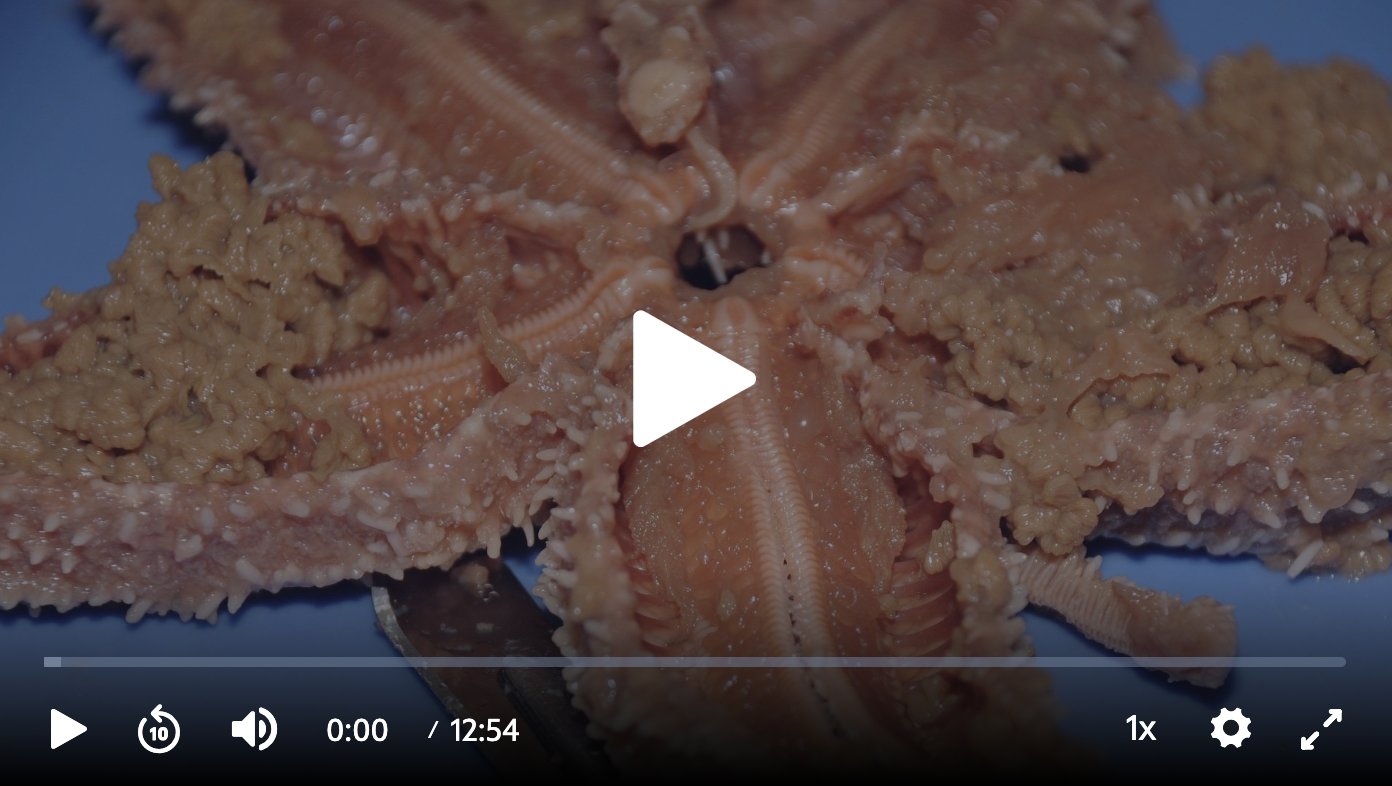
\includegraphics{images/Lab6_Seastar_Dissection_Video2.png}

\textbf{Seastar Quiz}

Complete the Seastar Quiz on \href{https://canvas.ubc.ca/}{Canvas}.

\hypertarget{phylum-chordata-perch-1}{%
\subsection*{Phylum Chordata-Perch}\label{phylum-chordata-perch-1}}
\addcontentsline{toc}{subsection}{Phylum Chordata-Perch}

Ribbons aren't just for presents! Perch lay their eggs in the form of ribbons.

\begin{figure}
\centering
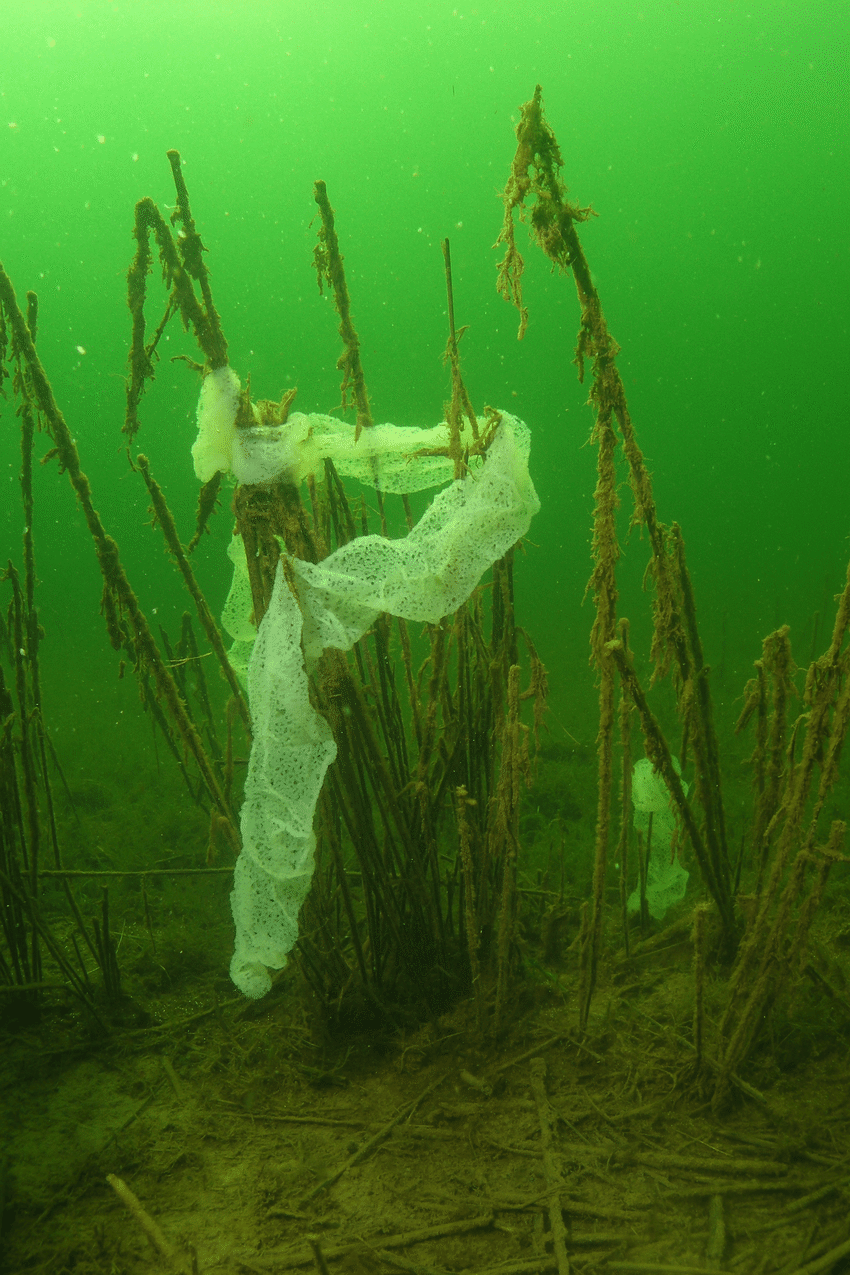
\includegraphics{images/Lab6_Egg_strand_perch.png}
\caption{Perch Egg Strand}
\end{figure}

Click \href{https://www.youtube.com/watch?v=T7xXfhOjtsU}{here} to see more!

\textbf{Perch Life Cycle}

\begin{figure}
\centering
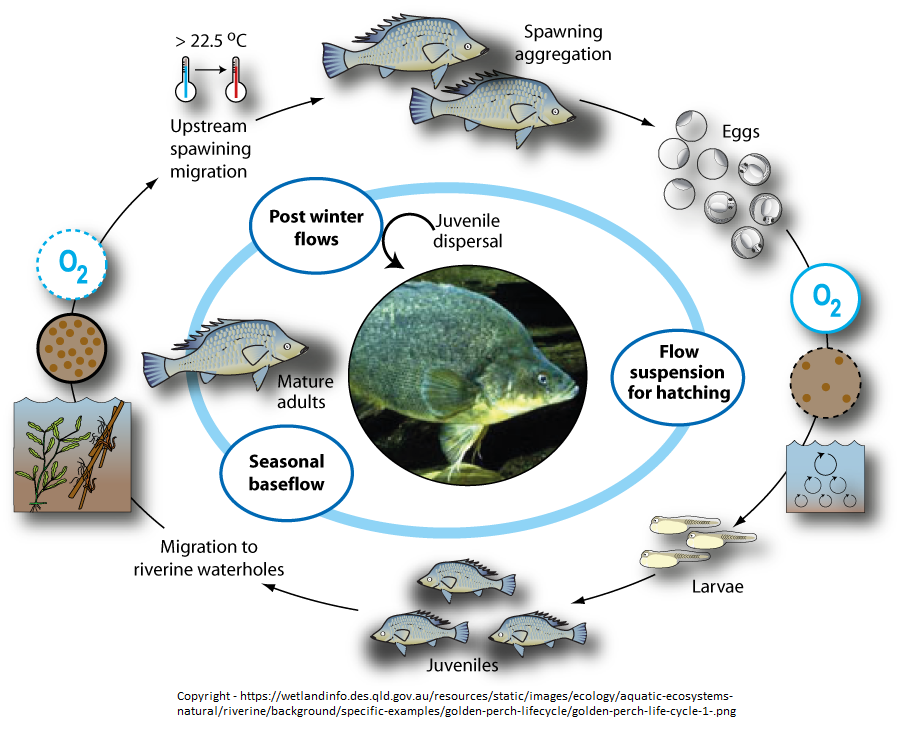
\includegraphics{images/Lab6_perch_life_cycle.png}
\caption{Perch Life Cycle}
\end{figure}

\textbf{Perch Dissection Guide \& Video}

Click \href{https://osf.io/download/hbkw9}{here} to download a copy of the Perch Dissection Guide.

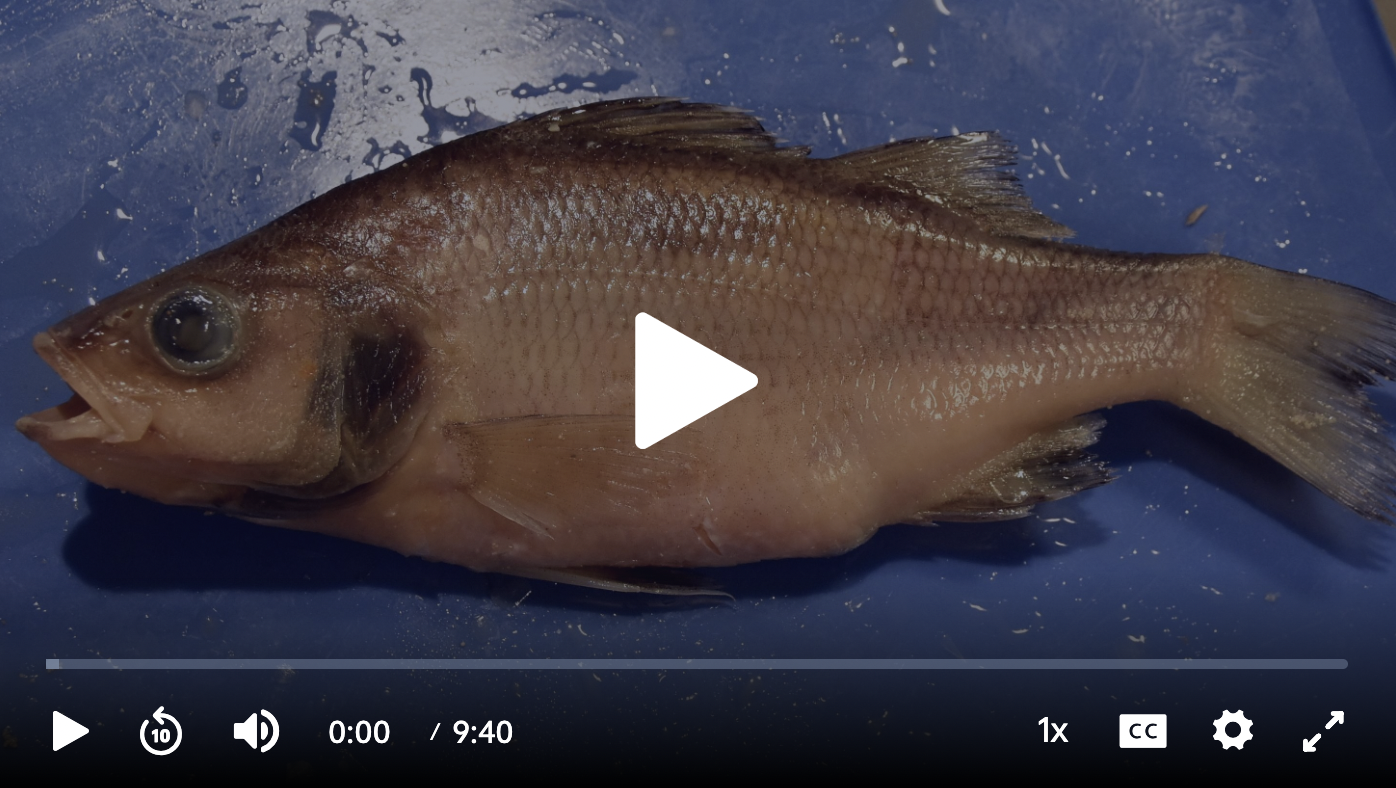
\includegraphics{images/Lab6_Perch_Dissection_Video1.png}

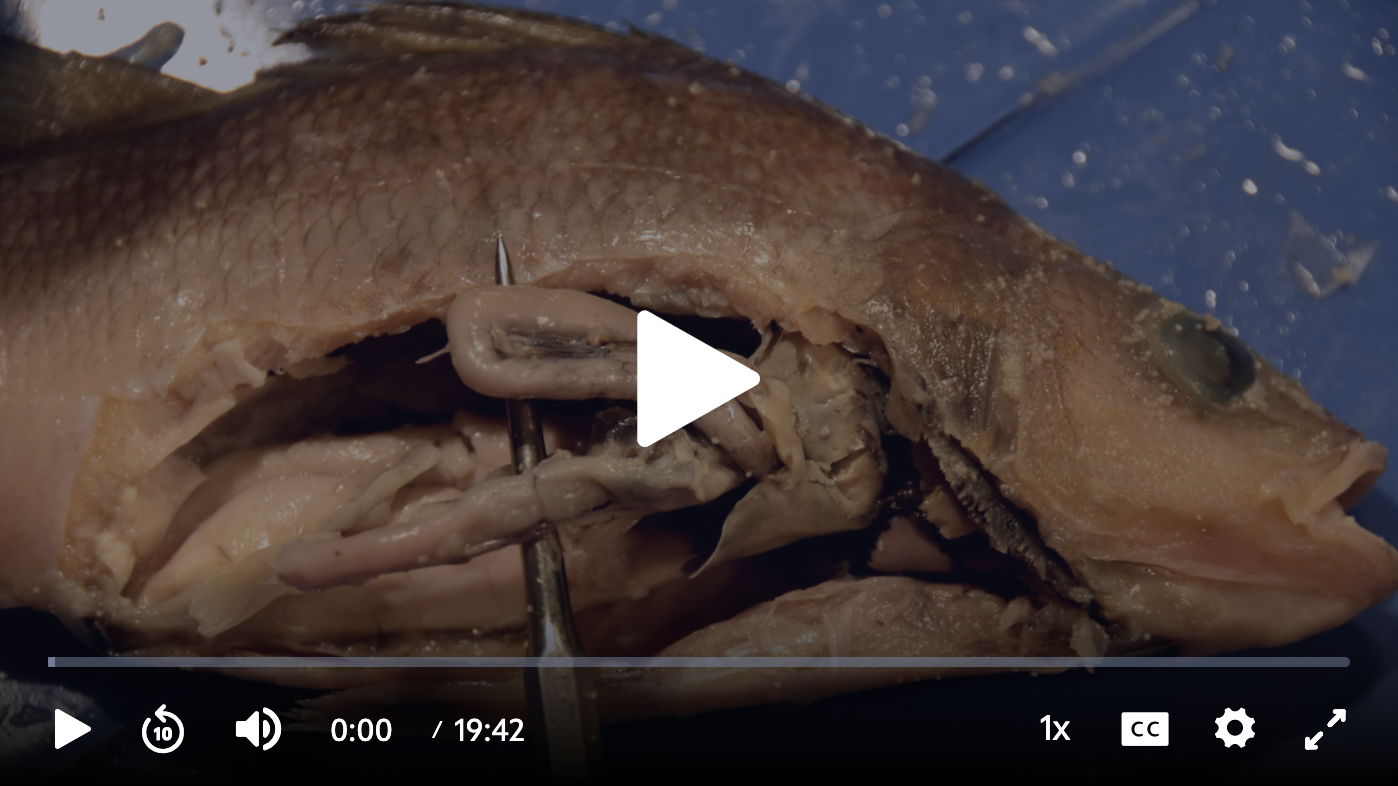
\includegraphics{images/Lab6_Perch_Dissection_Video2.png}

\textbf{Perch Quiz}

Complete the Perch Quiz on \href{https://canvas.ubc.ca/}{Canvas}.

\hypertarget{phylum-chordata-rat-1}{%
\subsection*{Phylum Chordata-Rat}\label{phylum-chordata-rat-1}}
\addcontentsline{toc}{subsection}{Phylum Chordata-Rat}

Rats can swim! And apparently climb up your toilet. Click \href{https://www.nationalgeographic.com/}{here} to check it out!

\textbf{Rat Life Cycle}

\begin{figure}
\centering
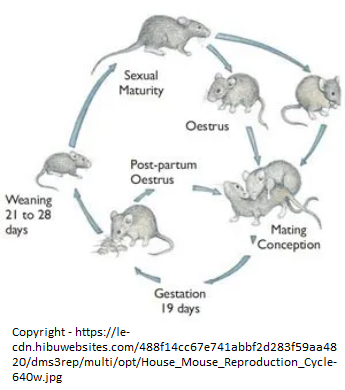
\includegraphics{images/Lab6_rat_life_cycle.png}
\caption{Rat Life Cycle}
\end{figure}

\textbf{Rat Dissection Guide \& Video}

Click \href{https://osf.io/download/72ztx}{here} to download a copy of the Rat Dissection Guide.

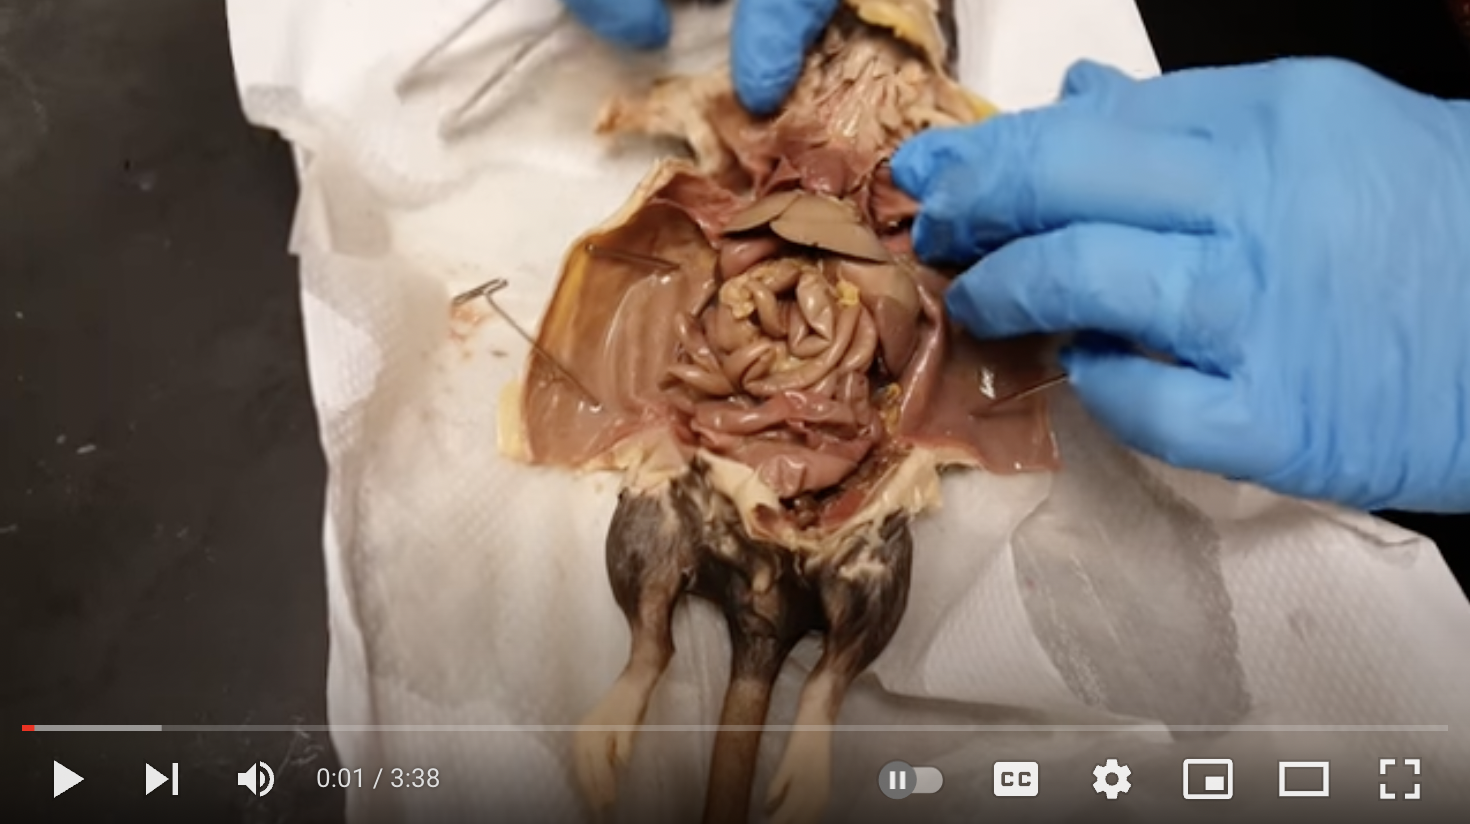
\includegraphics{images/Lab6_Rat_Dissection_Video.png}

\textbf{Rat Quiz}

Complete the Rat Quiz on \href{https://canvas.ubc.ca/}{Canvas}.

\hypertarget{part-lab-7}{%
\part*{Lab 7}\label{part-lab-7}}
\addcontentsline{toc}{part}{Lab 7}

\hypertarget{animal-systems-ii-part-two}{%
\chapter*{Animal Systems II: Part Two}\label{animal-systems-ii-part-two}}
\addcontentsline{toc}{chapter}{Animal Systems II: Part Two}

\emph{Last updated 2022-08-22}

\hypertarget{overview-of-the-week-3}{%
\subsection*{Overview of the Week}\label{overview-of-the-week-3}}
\addcontentsline{toc}{subsection}{Overview of the Week}

Breakdown:

\begin{enumerate}
\def\labelenumi{\arabic{enumi}.}
\tightlist
\item
  Come to lab ready on campus
\item
  Get assigned an animal and a group by your TA
\item
  Build a dissection presentation for your fellow students in the lab. Remember to add two errors to your presentation.
\item
  Submit Assignment \#5 before the end of the lab. Ensure all members have submitted a copy or those students missing a submission will receive a zero for the assignment and an absence score of 2.5.
  The last lab you spent a tremendous amount of time learning about echinoderms and chordates through videos, images, guides, and quizzes. Now, this week you will get to see these animals up close and personal!
\end{enumerate}

For this lab, you will be placed in groups and will be performing some dissections! Though not required, if you have lab coats please feel free to bring them along. All needed gloves and eye protection will be provided in the lab. For those of you who are not comfortable with dissections please know that you can still participate in the activity without having to do the actual dissection.

Make notes and work together as a team to learn about these groups. You and your group will create a dissection which you will then present to the other groups at your table. You will need to identify each structure and its function to your group. In order to make sure your peers are paying attention you must make up and/or incorrectly label two structures. The job of your peers is to now figure out which structure you presented incorrectly. Your TA will provide more details about the logistics of how this will work in the lab. In either case, have fun and enjoy the process!

\hypertarget{assignment-lab-7}{%
\chapter*{Assignment: Lab 7}\label{assignment-lab-7}}
\addcontentsline{toc}{chapter}{Assignment: Lab 7}

Click \href{https://osf.io/download/ze6ct}{here} to download a copy of Assignment 6.

\hypertarget{part-lab-8}{%
\part*{Lab 8}\label{part-lab-8}}
\addcontentsline{toc}{part}{Lab 8}

\hypertarget{fictional-animal-systems-project}{%
\chapter*{Fictional Animal Systems Project}\label{fictional-animal-systems-project}}
\addcontentsline{toc}{chapter}{Fictional Animal Systems Project}

\emph{Last updated 2022-08-22}

\emph{This assignment was developed from the article "The Fictional Animal Project: a Tool for Helping Students Integrate Body Systems". Adv. Physiol. Educ 41: 239-243 Blatch et al.~2017}

In the year 2146, biodiversity is dangerously low and the United Nations has developed a machine that randomly creates animals with varying designs for body systems and other physiological aspects. One example is a homeotherm with unidirectional ventilation, an open circulatory system, an excretory system that secretes only, and an incomplete digestive tract. In order to better understand the animals created and their ability to adapt to their environments, you have been asked to render a detailed anatomical ``blueprint'' of these animals, provide their scientific name, describe the relationships between the animal's form and function, between function and environment and provide a detailed diagram of its life cycle. This information will need to be presented to the ``Zoological Society'' in the form of a PowerPoint presentation. Using a random generator your TA will assign your animal design combination during this week's labs.

Learning goals:

\begin{itemize}
\tightlist
\item
  Understand system integration
\item
  Recognize the effects of adaptations relevant to the environment
\item
  Consider potential trade-offs and physiological constraints.
\item
  Solid understanding of the various animal systems which occur in nature and how they influence one another
\item
  Understand the anatomy involved in each of these systems within their designated animal
\end{itemize}

The presentation should fit onto one poster paper (approximately 24X36) and include the following information via diagrams/images and/or verbally:

\begin{itemize}
\tightlist
\item
  Blueprint of your animal; a detailed diagram of your organism including all systems and their relevant structures. Flow/current direction within the relevant systems should also be indicated. Remember to include a diagram of the exterior of your organism
\item
  The scientific name of your organism
\item
  A description of your animals' structure and function:

  \begin{itemize}
  \tightlist
  \item
    The description should align with your diagram
  \item
    Describe each system and how it works and be sure to include all structures relevant to that system
  \item
    Describe how each system interacts with each other
  \end{itemize}
\item
  A description of the habitat your organism would be found in how its structures are adapted for that environment
\item
  Detailed drawing of your organism's life cycle to include;

  \begin{itemize}
  \tightlist
  \item
    Any forms it takes on at the different stages of its cycle
  \item
    What part of the life cycle is haploid and diploid
  \item
    Where mitosis and meiosis occur
  \item
    Sexual or asexual reproduction
  \end{itemize}
\end{itemize}

Examples of types of questions to think about when working through your report:

\begin{enumerate}
\def\labelenumi{\arabic{enumi}.}
\tightlist
\item
  Does the circulatory fit with the respiratory system? Why or why not? Your explanation cannot be only because the combination exists in a real animal. Use your diagram to help you figure it out.
\item
  Does my organism's digestive system fit with the excretory system? Why or why not?
\item
  What might be an adaptive advantage of the combination of the systems you were assigned?
\item
  What might be an adaptive disadvantage of the combination of the systems you were assigned?
\item
  What constraints might be placed on the physiological process of each system by the combination of anatomic structures found in your animal?
\end{enumerate}

Additional instructions for the final project:

Describe an environment it would thrive in. Be specific. Explain why the animal thrives in that environment.

\hypertarget{animal-systems-presentation-prep}{%
\chapter*{Animal Systems Presentation Prep}\label{animal-systems-presentation-prep}}
\addcontentsline{toc}{chapter}{Animal Systems Presentation Prep}

You and your partner will be required to give a 5-minute presentation with each member presenting the same amount of time. Your presentation must be done using standard poster size paper 27 X 40 approximately. Your group will be given a grade for the quality of your oral presentation. It is important that you;

\begin{itemize}
\tightlist
\item
  Outline your talk as early as possible
\item
  Get together to organize and practice the presentation so the timing is accurate and you do not repeat information
\item
  Remember that your goal is to present material in a clear, succinct and interesting manner.
\end{itemize}

Suggestions for Content and Structure:

\begin{itemize}
\tightlist
\item
  Plan a strong, clear beginning and ending.
\item
  Provide a clear context for your work. Your introduction should include the objective and biological context of your study.
\item
  Include your hypotheses and prediction.
\item
  Present your materials and methods in a simple or streamlined manner. Keep it short and simple.
\end{itemize}

Presentation pointers for you:

\begin{itemize}
\tightlist
\item
  Practice over and over and over again until you can flow through the material without any hesitation. This will help ensure you have a handle on the material when you are nervous up at the front of the class. Take the opportunity to practice your presentation in the class
\item
  Get ready to perform. This is a performance! Know your lines and your subject.
\item
  Memorizing your lines can be problematic as you may start to sound too scripted. Use bullet points to help tell you what to talk about instead. Remember you are telling a story.

  \begin{itemize}
  \tightlist
  \item
    In order to help deal with nerves before a presentation work out slowing your breathing, visualize yourself giving a relaxed talk and even tell yourself you are confident. You may even want to ``power pose'' it! For those that don't watch
    Grey's Anatomy this is when you stand like superman or superwomen right before attempting something that makes you nervous. There are studies indicating this is very successful but at the very least it's not going to hurt right?
  \end{itemize}
\item
  Walk confidently to the front of the room to get you in the right frame of mind
\item
  Stand tall when you are up there and keep your chest lifted. Remember you totally got this!
\item
  Above all\ldots smile! You will instantly appear more relaxed and research shows that smiling can actually reduce your stress level. Plus, there is the added benefit of people enjoying the interaction more as you don't look like you are totally miserable up there ☺.
\item
  Speak up. People want to hear what you have to say so make sure they can.
\item
  Take your time. For you it's going to feel like its lasting forever but for your audience you may come across like you just had two coffees and a Red bull. Allow for those ``awkward'' pauses as for the audience it will actually sound more normal.
\item
  Talk to the audience and not your screen or cue cards. You should know the information so well that all you need is a quick bullet point to get you talking.
\item
  Keep to the time frame. This is where giving yourself lots of practice time will help out.
  Use the rubric provided to ensure you have covered all requirements of this assignment in order to attain the best possible outcome.
\end{itemize}

\hypertarget{part-lab-9}{%
\part*{Lab 9}\label{part-lab-9}}
\addcontentsline{toc}{part}{Lab 9}

\hypertarget{fictional-animal-systems-presentation}{%
\chapter*{Fictional Animal Systems Presentation}\label{fictional-animal-systems-presentation}}
\addcontentsline{toc}{chapter}{Fictional Animal Systems Presentation}

\emph{Last updated 2022-08-22}

\hypertarget{overview-of-the-week-4}{%
\subsection*{Overview of the Week}\label{overview-of-the-week-4}}
\addcontentsline{toc}{subsection}{Overview of the Week}

Your TA will pre-determine the order of your presentations and will let you know ahead of time. Please ensure you are ready to go. As this is the last lab and it requires a presentation during your scheduled lab section there will not be the option to submit 24 hours late.

\hypertarget{presentation-rubric}{%
\chapter*{Presentation Rubric}\label{presentation-rubric}}
\addcontentsline{toc}{chapter}{Presentation Rubric}

\textbf{Total /33}

\hypertarget{system-description}{%
\subsection*{System Description}\label{system-description}}
\addcontentsline{toc}{subsection}{System Description}

\textbf{/7}

\textbf{Criteria}

\begin{itemize}
\tightlist
\item
  All 5 systems were represented
\item
  At least 2 structures from each system were identified
\item
  The digestive system was clearly explained
\item
  The circulatory system was clearly explained
\item
  The excretory system was clearly explained
\item
  The respiratory system was clearly explained
\item
  The reproductive system was clearly explained
\end{itemize}

\begin{longtable}[]{@{}ll@{}}
\toprule()
Points & Criteria \\
\midrule()
\endhead
Exceeds Expectations 7 pts & All 7 criteria were met \\
Excellent 6 pts & 6 of the 7 criteria were met \\
Proficient 5 pts & 5 of the 7 criteria were met \\
Fair 4 pts & 4 of the 7 criteria were met \\
Unsatisfactory 3 pts & 3 of the 7 criteria were met \\
Poor 2 pts & 2 of the 7 criteria were met \\
Unacceptable 1 pt & Only 1 of the 7 criteria were met \\
Absent 0 pts & No criteria were met \\
\bottomrule()
\end{longtable}

\hypertarget{system-integration}{%
\subsection*{System Integration}\label{system-integration}}
\addcontentsline{toc}{subsection}{System Integration}

\textbf{/5}

\textbf{Criteria}

\begin{itemize}
\tightlist
\item
  Integration between the respiratory and circulatory system were explained well
\item
  Appropriate structures within the respiratory and circulatory were used when describing the compatibility
\item
  Integration between the excretory and digestive system were explained well
\item
  Appropriate structures within the digestive and excretory system were used when describing the compatibility
\item
  Explanation of the integration of these systems flowed well and was easy to follow
\end{itemize}

\begin{longtable}[]{@{}ll@{}}
\toprule()
Points & Criteria \\
\midrule()
\endhead
Excellent 5 pts & All 5 criteria were met \\
Proficient 4 pts & 4 of the 5 criteria were met \\
Satisfactory 3 pts & 3 of the 5 criteria were met \\
Poor 2 pts & 2 of the 5 criteria were met \\
Unacceptable 1 pt & Only 1 of the 5 criteria were met \\
Absent 0 pts & No criteria were met \\
\bottomrule()
\end{longtable}

\hypertarget{life-cycle}{%
\subsection*{Life Cycle}\label{life-cycle}}
\addcontentsline{toc}{subsection}{Life Cycle}

\textbf{/6}

\textbf{Criteria}

\begin{itemize}
\tightlist
\item
  All relevant reproductive structures have been identified
\item
  Type of reproduction has been made clear
\item
  Full description of the reproductive process has been provided
\item
  Life cycle has been provided and explained
\item
  All relevant structures of the life cycle have been properly identified
\item
  Ploidy of structures has been clearly shown
\end{itemize}

\begin{longtable}[]{@{}ll@{}}
\toprule()
Points & Criteria \\
\midrule()
\endhead
Excellent 6 pts & All criteria were met \\
Proficient 5 pts & 5 of the 6 criteria were met \\
Good 4 pts & 4 of the 6 criteria were met \\
Satisfactory 3 pts & 3 of the 6 criteria were met \\
Poor 2 pts & 2 of the 6 criteria were met \\
Unacceptable 1 pt & Only 1 of the 6 criteria were met \\
Absent 0 pts & No criteria were met \\
\bottomrule()
\end{longtable}

\hypertarget{environment-and-system-compatability}{%
\subsection*{Environment and System Compatability}\label{environment-and-system-compatability}}
\addcontentsline{toc}{subsection}{Environment and System Compatability}

\textbf{/4}

\textbf{Criteria}

\begin{itemize}
\tightlist
\item
  Clearly explains how the respiratory system of the animal works with its environment
\item
  Clearly explains how the circulatory system of the animal works with its environment
\item
  Clearly explains how the digestive system of the animal works with its environment
\item
  Clearly explains who the excretory system of the animal works with its environment
\end{itemize}

\begin{longtable}[]{@{}ll@{}}
\toprule()
Points & Criteria \\
\midrule()
\endhead
Excellent 4 pts & All criteria were met \\
Proficient 3 pts & 3 of the 4 criteria were met \\
Satisfactory 2 pts & 2 of the 4 criteria were met \\
Unacceptable 1 pt & Only 1 of the 4 criteria were met \\
Absent 0 pts & No criteria were met \\
\bottomrule()
\end{longtable}

\hypertarget{environment---morphological-and-behavioural-adaptations}{%
\subsection*{Environment - Morphological and Behavioural Adaptations}\label{environment---morphological-and-behavioural-adaptations}}
\addcontentsline{toc}{subsection}{Environment - Morphological and Behavioural Adaptations}

\textbf{/3}

\textbf{Criteria}

\begin{itemize}
\tightlist
\item
  Clear description of how the animal has adapted to live in its environment behaviorally
\item
  Clear description of how the animals had adapted physically (body structure, types of appendages, etc) to live in their environment
\item
  Structures involved in helping to adapt the animal to its environment are clearly articulated
\end{itemize}

\begin{longtable}[]{@{}ll@{}}
\toprule()
Points & Criteria \\
\midrule()
\endhead
Excellent 3 pts & All criteria were met \\
Satisfactory 2 pts & 2 of the 3 criteria were met \\
Unacceptable 1 pt & Only 1 of the 3 criteria were met \\
Absent 0 pts & No criteria were met \\
\bottomrule()
\end{longtable}

\hypertarget{presentation}{%
\subsection*{Presentation}\label{presentation}}
\addcontentsline{toc}{subsection}{Presentation}

\textbf{/5}

\textbf{Criteria}

\begin{itemize}
\tightlist
\item
  Presentation was clear and easy to follow
\item
  Volume of all presenters was appropriate
\item
  Presenters shared in the presentation equally
\item
  All presenters were engaging and showed enthusiasm for their project
\item
  All presenters displayed a solid understanding of their animal and the corresponding systems
\end{itemize}

\begin{longtable}[]{@{}ll@{}}
\toprule()
Points & Criteria \\
\midrule()
\endhead
Excellent 5 pts & All 5 criteria were met \\
Proficient 4 pts & 4 of the 5 criteria were met \\
Fair 3 pts & 3 of the 5 criteria were met \\
Unsatisfactory 2 pts & 2 of the 5 criteria were met \\
Unacceptable 1 pt & Only 1 of the 5 criteria were met \\
Absent 0 pts & No criteria were met \\
\bottomrule()
\end{longtable}

\hypertarget{plagiarism-and-in-text-citations}{%
\subsection*{Plagiarism and In-Text Citations}\label{plagiarism-and-in-text-citations}}
\addcontentsline{toc}{subsection}{Plagiarism and In-Text Citations}

\textbf{/3}

\textbf{Criteria}

\begin{itemize}
\tightlist
\item
  No plagiarism of any kind
\item
  In-text citations were used when appropriate and followed APA format
\item
  References were provided
\end{itemize}

\begin{longtable}[]{@{}ll@{}}
\toprule()
Points & Criteria \\
\midrule()
\endhead
Excellent 3 pts & All criteria were met \\
Satisfactory 2 pts & 2 of the 3 criteria were met \\
Unacceptable 1 pt & Only 1 of the 3 criteria were met \\
Absent 0 pts & No criteria were met \\
\bottomrule()
\end{longtable}

\end{document}
